%----------------------------------------------------------------%
% Bachelorarbeit
%----------------------------------------------------------------%
%----------------------------------------------------------------%
%																																 %
% Datei: header.tex																							 %
%----------------------------------------------------------------%

\documentclass[pagesize=pdftex,paper=a4,fontsize=12pt,abstract=true,twoside,openright]{scrreprt}

\pagestyle{headings}

\usepackage[latin9]{inputenc}

\usepackage[onehalfspacing]{setspace}

\usepackage{ngerman}

\usepackage{graphics, graphicx,wrapfig}
\usepackage{fancybox}
\usepackage{picinpar,varioref}
\usepackage{capt-of}
\usepackage{caption}
\usepackage{moreverb}
\usepackage{rotating}
\usepackage{enumerate}

\usepackage{longtable}

\usepackage{color}

\usepackage{colortbl}

\usepackage{hhline}

\usepackage{listings}

\usepackage{bibgerm}

\usepackage[toc,acronym,nonumberlist]{glossaries}

\makeglossaries

\parindent 0pt

\parskip 12pt


\begin{document}
\pagenumbering{Roman}
\newacronym{xml}{XML}{Extensible Markup Language}
\newacronym{gui}{GUI}{Graphical User Interface}
\newacronym{opengl}{OpenGL}{Open Graphics Library}
\newacronym{swt}{SWT}{Standard Widget Toolkit}
\newacronym{dom}{DOM}{Document Object Model}
\newacronym{sax}{SAX}{Simple Application Programming Interface for Extensible Markup Language}
\newacronym{jme}{jME}{Java Monkey Engine}
\newacronym{png}{PNG}{Portable Network Graphics}
\newacronym{rss}{RSS}{Really Simple Syndication}
\newacronym{pdf}{PDF}{Portable Document Format}
\newacronym{jdl}{JDL}{Joint Directors of Laboratories}
\newacronym{mac}{MAC}{Media Access Control}
\newacronym{ndp}{NDP}{Neighbor Discovery Protocol}
\newacronym{ip}{IP}{Internet Protocol}
\newacronym{lwjgl}{LWJGL}{Lightweight Java Game Library}


%----------------------------------------------------------------%
% titelseite.tex																					       %
%----------------------------------------------------------------%
\thispagestyle{empty}
\vspace*{-2ex}

\centerline{
\includegraphics[width=7cm]{signet}}
\vspace{3cm}

\begin{center}
\begin{minipage}[t]{10cm}      %% Anfang Sichtfenster
\begin{center}

{\bf  Visualisierung von multisensor Daten zur Vorbereitung von Datenfusion am Beispiel einer milit�rischen Lage }\\[5mm]
Bachelor Thesis von \\
Stephan Tzschoppe \\
1006374 \\[5mm]
UniBwM -- IB 16/2009 \\
\end{center}
\end{minipage}                 %% Ende Sichtfenster

\vspace*{2cm}
Aufgabenstellung:\\
Prof. Dr. Stefan Pickl\\[1cm]
Betreuung:\\
Dipl.-Inf. Marco Schuler \\[12mm]

Institut f�r Theoretische Informatik, \\
Mathematik und Operations Research \\
Fakult�t f�r Informatik \\
Universit�t der Bundeswehr M�nchen\\[5mm]

Neubiberg \\
18.12.2009
\end{center}

\cleardoublepage


\tableofcontents

%Resets the acronyms after abstract
\glsresetall
\onehalfspacing
%----------------------------------------------------------------%
% einleitung.tex																					       %
%----------------------------------------------------------------%
\chapter{Einleitung}

\section{Motivation}
Wir leben in einer Zeit stetig voranschreitender Technologisierung. Dies �u�ert sich f�r jeden sichtbar auf vielerlei Art und Weise. Massenspeicher mit vor Jahren noch unvorstellbaren Kapazit�ten, stetig wachsende Prozessorleistung und massiver Fortschritt in der Daten�bertragung sind hier nur als Beispiele zu nennen. Solche Entwicklungen sind es, die das Sammeln, Verarbeiten und Speichern von riesigen Datenmengen erst erm�glichen.  Diesen Fortschritt gilt es zu nutzen und auf m�gliche Anwendungsfelder auszuweiten. 

\label{motivation}
Betrachtet man ein Schlachtfeld, sei es im Rahmen einer �bung, einer kriegerischen Auseinandersetzung oder eines Konflikts, so werden auch hier Informationen gesammelt und ausgewertet. Man stelle sich folgende Situation vor: Drei eigene Panzer bewegen sich durch das Gel�nde. Pl�tzlich kl�ren sie zwei feindliche Fahrzeuge auf. Jeder einzelne eigene Panzer setzt eine Meldung ab und beschreibt, was er sieht. Dies f�hrt zu sechs Meldungen. Der S2\footnote{Der S2-Offizier ist verantwortlich f�r die Milit�rische Sicherheit, Milit�risches Nachrichtenwesen mit Aufkl�rung und Zielfindung, elektronisch Kampff�hrung und eben die Wehrlage}-Offizier muss nun aus diesen Meldungen ein Lagebild erstellen. Dabei gilt es aus der vorhandenen (teilweise redundanten) Information die zwei statt sechs feindliche Fahrzeuge zu erkennen. 

F�r das geschilderte Beispiel scheint es nicht notwendig, diese Informationsauswertung zu automatisieren. In der Realit�t hingegen \footnote{Ein Panzerbataillon der Bundeswehr umfasst zum Beispiel ungef�hr 40 Kampfpanzer} erfordert es viel Zeit, diese Arbeit zu erledigen. Und genau dies ist ein gro�es Problem, denn je �lter die Lageinformation ist, umso weniger aussagekr�ftig ist sie. Entscheidungen, die darauf basierend getroffen werden, k�nnen daraufhin falsch oder unverh�ltnism��ig sein. Um diesen Missstand zu beseitigen, gilt es, den S2-Offizier bei seiner Arbeit technisch zu unterst�tzen.

\section{Ziel der Arbeit}

Eine technische Unterst�tzung kann in unterschiedlichen Abstufungen geschehen. So k�nnen die separaten Meldungen zu einer gro�en Meldung zusammengefasst werden. Dies ist aber nicht sonderlich hilfreich, wenn zum Beispiel aus vielen einzelnen Datens�tzen einfach eine zusammenh�ngende Datensammlung erstellt wird. Denn wenn diese in einem textuellen Format vorliegt, ist sie von einem Menschen nur schwer zu verstehen. Weiterhin k�nnen die auftretenden Redundanzen nicht einfach erfasst, geschweige denn �berhaupt genutzt werden.

Aus diesem Grund m�chte ich mich in dieser Arbeit mit M�glichkeiten auseinandersetzen, eine menschenlesbare Sicht auf multisensorische Daten zu erstellen. Zum Einen sollen Visualisierungsm�glichkeiten aufgezeigt werden. Weiterhin soll bei unterschiedlichen Ans�tzen, eine Bewertung  dieser vorgenommen werden.

Ergebnis dieser Betrachtungen wird ein Framework zur Darstellung multisensorischer Daten. Dieses verwende ich dann prototypisch dazu, die eingangs erw�hnte Problemstellung des S2-Offiziers zu bearbeiten und ihm eine, f�r seine Lageerstellung hilfreiche, Sicht auf die eingehenden Meldungen zu geben.

Die Erweiterbarkeit des Frameworks soll durch dessen Verwendung zur Darstellung von NDP [ABK] Daten gezeigt werden.


\section{Aufbau der Arbeit}

\chapter{Verwendete Technologien}
\label{ch:technologien}
In diesem Kapitel werden die wichtigsten Technologien, die im Laufe der Arbeit verwendet werden, vorgestellt und erl�utert.

\section{Java}
Am Anfang der Arbeit stand die Wahl der Programmiersprache, die f�r die Implementierung verwendet werden sollte. Java in der Version 1.6 bot sich aus mehren Gr�nden an.

Auf der einen Seite sprach ein ganz pragmatischer Grund daf�r: Da Java im Rahmen der Vorlesung �ber Objektorientierte Programmierung gelehrt wurde, entfiel die Einarbeitungszeit. Auf der anderen Seite gibt es aber weitere Gr�nde f�r die Wahl. An die prototypische Implementierung wurde die Anforderung der Plattformunabh�ngigkeit gestellt. Dies spricht f�r die Wahl einer Sprache, die auf einer virtuellen Maschine basiert. Im Gegensatz zu einem Java-Programm m�sste ein in C++ geschriebenes auf einem anderen Rechner neu kompiliert werden. Dies erh�ht den Installationsaufwand und ist keine echte Unabh�ngigkeit.

Unter den Sprachen, die auf einer Virtuellen Maschine basieren f�llt aus Gr�nden der Plattformunabh�ngigkeit die .Net-Familie aus, da es sich hier um Microsoft- und somit betriebssystemspezifische Sprachen handelt. Weitere Gr�nde f�r die Wahl von Java waren existierende Klassenbibliotheken f�r die Verwendung von XML (siehe \ref{ch:xml}) und die Arbeit mit OpenGL als Programmierschnittstelle f�r die dreidimensional Visualisierung.

Ein Nachteil von Java ist die Umsetzung von GUI-Elementen. Zwar gibt es mit Swing und SWT leistungsf�hige Bibliotheken, aber das Layout der grafischen Benutzeroberfl�che ansprechend zu gestalten, stellt sich damit als schwierig heraus. F�r die Umsetzung der grafischen Benutzeroberfl�che wurde Swing gew�hlt, da es Bestandteil der mit Java ausgelieferten Klassenbibliothek ist

Weiterhin ist die Verwendung von Java f�r die Arbeit mit 3D-Grafik umstritten (siehe \cite{killer}). Ein gro�er Kritikpunkt ist dabei der Geschwindigkeitsverlust, der sich aus dem Interpretieren des Programms durch die Virtuelle Maschine ergibt. Wie stark dieser ins Gewicht f�llt, ist umstritten. Da Geschwindigkeit f�r diese Arbeit aber nicht Ausschlaggebend ist, kann dieser Kritikpunkt vernachl�ssigt werden.
\section{XML}
\label{ch:xml}
Die Daten f�r das Testen der prototypischen Entwicklung stammen von einem Gefechtssimulator. Sie sind im XML-Format abgespeichert. Um mit diesen Daten in Java arbeiten zu k�nnen, m�ssen sie in Java-Klassen �berf�hrt werden. An dieser Stelle kamen zwei M�glichkeiten in Frage: Auf der einen Seite h�tte nur die prototypische Implementierung, die mit den Daten arbeitet, diese eingelesen. Auf der anderen Seite konnte die Funktionalit�t, aus XML-Dateien zu laden, auch in das entwickelte Framework integriert werden.

Weil sich XML f�r einen plattform- und implementierungsunabh�ngigen Datenaustausch eignet und heute zu diesem Zweck ein Quasistandart ist [CITE]. Fiel die Entscheidung, das Laden von Daten im XML-Format im Framework zu implementieren. Die gew�hlte Programmiersprache eignete sich f�r diesen Zweck besonders gut, da bereits fertige Parser-Bibliotheken mitgeliefert werden.

Hier standen DOM und SAX zur Auswahl. Beide haben Vor- und Nachteile. Welche Implementierung gew�hlt wird, h�ngt vom zu l�senden Problem ab. Wird mit gro�en Datenmengen gearbeitet und m�ssen diese oft neu geladen werden, ist SAX im Vorteil, weil es sich dabei um eine sehr performante Umsetzung handelt. Ein gro�er Nachteil ist die eingeschr�nkte Traversierbarkeit der Daten. Das h�ngt mit der Arbeitsweise des Parsers zusammen. Er arbeitet ereignisgesteuert. Das bedeutet, die XML-Datei wird sequentiell gelesen. Wird beispielsweise ein Element gefunden, wird eine Methode zur Verarbeitung von Elementen aufgerufen. Somit kann bei der Verarbeitung kein R�ckschluss auf die Position eines Elements in der XML-Datei geschlossen werden. Genauso wenig kann auf Vorg�nger, Nachfolger unter Unterelemente explizit zugegriffen werden.

Der gro�e Vorteil des DOM-Parsers ist eben die bei SAX nicht vorhandene Traversierbarkeit. Der Parser erzeugt beim Einlesen der XML-Datei einen Baum. F�r jedes strukturelle Element der Daten wird ein Knoten erzeugt. Ein XML-Element ist ein Bespiel f�r einen solchen Knoten, aber auch ein Attribut. Auf diese Art und Weise ist es zum einen m�glich, sich komfortabel durch die Daten zu bewegen. Weiterhin ist es so m�glich, das Lesen von XML-Dateien in das erstellte Framework zu integrieren und f�r jede Implementierung mit lediglich geringem Implementierungsaufwand eine Leseroutine umzusetzen. Das Framework ist dann in der Verantwortung die Elemente zu extrahieren, die einen Datensatz darstellen. Der Anwender des Frameworks bekommt dann die Knoten der Datens�tze und liest eigenst�ndig die von ihm ben�tigten Informationen aus. Aus diesem Grund wurde DOM f�r diese Arbeit ausgew�hlt.

Die Tatsache, dass DOM nicht so sehr f�r gro�e Datenmengen geeignet ist, weil das Erzeugen der Baumstruktur vor allem speicherplatzintensiv ist. Dieser Nachteil wird aber zum Wohle des einfacheren Umgangs in Kauf genommen.

\section{jMonkeyEngine}

\section{Google Code}
Bei der Entwicklung des praktischen Anteils dieser Arbeit bestand die Notwendigkeit, die erstellten Daten sicher abzulegen. Daf�r eignet sich unter anderem die Arbeit auf einem Terminal-Server, wir er von der Universit�t der Bundeswehr angeboten wird. Dies erm�glicht, von unterschiedlichen Orten und an unterschiedlichen Rechnern zu arbeiten. Nachteil dieser L�sung ist jedoch, dass ein Speichern unterschiedlicher Versionen des erstellten Programms und auch dieser Arbeit nur schwer m�glich ist.

Aus diesem Grund wurde f�r das im Rahmen dieser Arbeit erstellte Programm, aber auch f�r die schriftliche Ausarbeitung, ein Versionierungssystem verwendet. Aus der Lehre bereits bekannt war Subversion. Es wurde auch hier wegen der nicht mehr notwendigen Einarbeitung gew�hlt. 

Google stellt auf seinem Portal GoogleCode die M�glichkeit bereit, eine Projekt mit Hilfe von Subversion zu versionieren. Dieser sogenannte \emph{Project Hosting Service} hat zudem noch weitere Vorteile als nur eine komfortable Datensicherung: Der Projektstand kann online dokumentiert werden. Somit wird es m�glich, den Betreuer dieser Arbeit auf dem neusten Stand zu halten. Er kann �ber das Abonnieren eines RSS-Feeds jederzeit �nderungen Nachverfolgen. Weiterhin bietet Google ein Wiki an, was die Vorstellung und die Dokumentation des Programms erm�glicht. Zus�tzlich gibt es eine Downloadverwaltung in der Testversionen Screenshots und �hnliches zur Verf�gung gestellt werden k�nnen.

Wie oben angesprochen, wurde nicht nur der praktische Teil der Arbeit, also der Quellcode, �ber das Versionierungssystem gesichert. Auch die schriftliche Ausarbeitung in Form des Rohzustands (\TeX-Dateien) und des fertigen PDF-Kompilats wurde auf im Googleprojekt gespeichert.

Zusammenfassend sind die Vorteile des oben geschilderten Vorgehens, dass der Quellcode und die schriftliche Ausarbeitung zuverl�ssig gesichert werden konnten.  Der Zugriff auf diese war ortsunabh�ngig �ber das Internet m�glich. Mit Hilfe der Versionierung konnte nach Experimenten auf stabile Versionen zur�ckgegriffen werden. Durch RSS-Feeds war es dem Betreuer jederzeit m�glich, den aktuellen Stand der Arbeit zu betrachten und die im Downloadbereich befindliche Version zu testen.


%----------------------------------------------------------------%
% theorie.tex																			       %
%----------------------------------------------------------------%

\chapter{Multisensorische Daten und ihre Visualisierung}
\label{ch:theorie}

In diesem Kapitel soll zuerst der Zusammenhang zwischen dem Thema dieser Arbeit und den daf�r relevanten theoretischen Grundlagen dargelegt werden. Darauf folgend sollen M�glichkeiten der Datenvisualisierung aufgezeigt. Einige davon sind in der prototypischen Implementierung umgesetzt, andere wurden nicht aufgenommen. Die Gr�nde daf�r sollen an geeigneter Stelle dargelegt werden.

\section{Theoretische Einordnung}
\label{sec:TheoretischeEinordnung}
In diesem Abschnitt soll die  theoretische Einordnung der Arbeit erfolgen. An erster Stelle steht dabei die Erl�uterung multisensorischer Daten anhand eines einfachen Beispiels. Anschlie�end soll mit dessen Hilfe der Begriff \emph{Multisensor Data Fusion} definiert und der praktische Teil dieser Arbeit in den theoretischen Kontext eingeordnet werden.

\subsection{Multisensorische Daten}
\label{sec:EigenschaftenVonMultisensorischenDaten}
Der Begriff der \emph{multisensorischen Daten} existiert in der Literatur nicht losgel�st. Interessant ist er nur in Verbindung der Fusion von Daten. Trotzdem soll an dieser Stelle eine kurze begriffliche Betrachtung stehen.

\label{beispiel}
Ein kleines Beispiel verdeutlicht sehr gut, worum es hier geht: Man stelle sich einen Tisch vor, auf dem zwei brennende Kerzen stehen. Davor befinden sich drei Beobachter. Jeder soll unabh�ngig von den anderen jeden Gegenstand, den er sieht, auf je einem Blatt Papier beschreiben. Bei den entstehenden Dokumenten handelt es sich um eine Form von multisensorischen Daten. Ein Datum ist dabei eine Beschreibung eines Gegenstandes. Ein Sensor ist jeweils einer der Beobachter.  Dies ist ein Ansatz, sich der Thematik zu n�hern. 

Ein anderer Ansatz k�nnte bei selbem Aufbau mit einer Person gemacht werden. Denn der Mensch, oder besser seine Sinne liefert schon multisensorische Daten. Die Person sieht eine Lichtquelle und f�hlt eine Hitzequelle. Diese beiden Beobachtungen sind die Daten, die Sensoren sind Tastsinn und Sehsinn.

Multisensorische Daten wie oben geschildert sind aber in der Theorie und Praxis nicht von Bedeutung, wenn sie f�r sich genommen werden. Schl�ssige Informationen daraus sind n�mlich nicht m�glich, ohne die Eingangsdaten zu interpretieren. Dieser Vorgang, man spricht von \emph{Multisensor Data Fusion}, soll in Abschnitt \ref{sec:MultisensorFusion} erl�utert werden.
\paragraph{Vorteile}
\label{sec:Vorteile}
In \cite{MDFLLINAS} werden neun Vorteile von multisensorischen Systemen (und den von ihnen gelieferten Daten) aufgez�hlt, die hier in Auswahl sinngem�� wiedergegeben werden sollen:

\begin{enumerate}
	\item \textbf{Robustheit:} Informationen k�nnen weiter gesammelt werden, auch wenn ein oder mehrere Sensoren keine Daten mehr liefern.

	\item \textbf{R\protect\"aumlich weitreichende Abdeckung:} Daten, die vielleicht nur von einem ein paar Sensoren gesehen werden, w�rden nicht entdeckt, wenn nur ein einzelner Sensor an der falschen Stelle steht.

	\item \textbf{Zeitlich weitreichende Abdeckung:} Nicht jeder Sensor steht zu jeder Zeit zur Verf�gung. Bei zeitlichem Versatz und �berlappung kann eine dauerhafte Datensammlung betrieben werden.

	\item \textbf{Gesteigerte Informationssicherheit:} Wird ein Datum durch mehrere Sensoren erfasst, verringert sich die Wahrscheinlichkeit eines Messfehlers.

	\item \textbf{Erh�hte Informationsdichte:} Die Aufl�sung, mit der mehrer Sensoren ein Gebiet abtasten k�nnen, ist h�her als die Aufl�sung eines einzelnen Sensors.
\end{enumerate}

Diese Reihe von Vorteilen zeigt, dass die Datensammlung mit mehreren Sensoren durchaus betrieben werden sollte. Die entstehenden Daten bieten vor allem durch ihre Redundanzen  mehr und sichere Informationen als die eines einzelnen Sensors.

\paragraph{Nachteile}
\label{sec:Nachteile}
Die oben angesprochene Redundanz ist zugleich der gr��te Nachteil von multisensorischen Daten. Wie sich das �u�ert, sei noch mal an dem in Abschnitt \ref{beispiel} eingef�hrten Beispiel erl�utert: Die schriftlich gesammelten Daten der drei Beobachter werden an eine Person weitergegeben, die sich zum Zeitpunkt der Beobachtungen an einem anderen Ort aufhielt. Diese Person soll aus den Daten schlie�en, was sich auf dem Tisch befand. Sie hat dabei keine Informationen, welche Daten von welchem Beobachter stammen. Ebenfalls ist unbekannt, wie viele Beobachter �berhaupt beteiligt waren.

Aus den Daten k�nnte die auswertende Person schlie�en, dass sechs Kerzen auf dem Tisch befanden. Dies ist ein v�llig falsches Bild und der Grund f�r die Fehlinterpretation ist die Redundanz der Daten, die nicht beseitigt wurde. Nur wenn Datens�tze, die zu einem realen Objekt geh�ren, zusammengef�hrt werden, kann man die Vorteile von multisensorischen Daten nutzen.


 
\subsection{Multisensor Data Fusion}
\label{sec:MultisensorFusion}
Um die Redundanz aus den von mehreren Sensoren gewonnenen Daten herauszufiltern, m�ssen die Datens�tze fusioniert werden. Die theoretischen Hintergr�nde zu dem \emph{Multisensor Data Fusion} genannten Vorgang sind im Folgenden dargelegt. 
\paragraph{Begriffsbestimmung}
\label{sec:Begriffsbestimmung}
Der Begriff \emph{Fusion} kann wie folgt definiert werden:
\begin{quote}
		"`[Fusion is] the integration of information from multiple sources to procedure specific and comprehensive unified data about an entity"' \protect\cite{fusionintroduction}
\end{quote}


Aus dieser Definition kann geschlossen werden, dass durch die Fusion von Daten nicht nur ungewollte Redundanzen beseitigt werden k�nnen. Es wird auch ein Informationsgewinn erreicht, der auf den Vorteilen mehrerer Sensoren beruht (siehe \ref{sec:Vorteile}), frei nach Aristoteles: "`Das Ganze ist mehr als die Summe seiner Teile."'. Datenfusion ist ein Prozess, der nach \cite{MDFLLINAS} drei Aspekte in sich vereint:

\begin{itemize}
	\item Datenfusion ist ein Prozess, der auf Unterschiedlichen Ebenen Abl�uft. Die unterschiedlichen \emph{Level} beziehen sich auf den unterschiedlich hohen Abstraktionsgrad der Daten. Sie sind im n�chsten Abschnitt beschrieben.

	\item Datenfusion schlie�t die Vorg�nge der Erkennung, Assoziation, Korrelation, Beurteilung und Vereinigung von Daten ein.

	\item Das Ergebnis des Prozesses umfasst Ansch�tzung zu Identifikation und Eigenschaften von Daten bis hin zu Erkenntnissen �ber komplexe Lagen oder Situationen.
\end{itemize}

Datenfusion findet in vielen Breichen, vor allem beim Milit�r, Anwendung. Beispiele werden in \cite{mathfusion} aufgezeigt. Dazu geh�ren unter anderem die �berwachung der Meere, Luftverteidigung (durch Boden- und durch Lufteinheiten), Aufkl�rung auf dem Gefechtsfeld, strategische Luftaufkl�rung, Suche nach Bodensch�tzen, Diagnostik in der Medizin und vor allem Robotik. 

\paragraph{Fusion Level}
\label{sec:FusionLevel}

Die Datenfusion kann, wie oben bereits angesprochen, in insgesamt f�nf unterschiedliche Ebenen unterteilt werden. Grundlage daf�r ist das vom Joint Directors of Laboratories (JDL) entwickelte Prozessmodell (\cite{mathfusion}). Der Abstraktionsgrad erh�ht sich mit aufsteigender Stufennummer. F�r die praktische Anwendung von Datenfusion sind vor allem die ersten drei Stufen relevant.

\begin{itemize}
	\item Level 1 -- Object Assessment: Bestimmung der Identit�t und der Eigenschaften eines Objekts

	\item Level 2 -- Situation Assessment: Bewertung einer Lage einschlie�lich der Bestimmung von Beziehungen zwischen Objekten, zwischen den Objekten und ihrer Umgebung und ihrer Bedeutung.

	\item Level 3 -- Impact Assessment: Entwicklung der gegenw�rtigen Lage in die Zukunft und damit verbundene Auswirkungen (zum Beispiel Bedrohungen)
\end{itemize}

Die in dieser Arbeit umgesetzte Fusion durch Visualisierung soll im n�chsten Abschnitt in dieses Modell eingeordnet werden.


\paragraph{Einordnung der Arbeit}
\label{sec:EinordnungDerArbeit}

Der Sachverhalt des S2-Offiziers, der Meldungen aus dem Gefechtsfeld bekommt, und diese zu einer gro�en Lage zusammenf�gt k�nnte sehr einfach in die zweite Ebene eingeordnet werden, schlie�lich erstellt er eine Lage. Diese Einsch�tzung ist jedoch falsch, denn um auf dieses Level zu kommen, muss die Redundanz in den Objekten beseitigt sein, und genau das ist schlie�lich erst das Ziel. Dies ist das erste Problem bei der Einordnung.

Ein weiteres Problem entsteht durch die Sensoren, welche die Daten f�r die Visualisierung und damit f�r die Fusion liefern. Es handelt sich (in der Realit�t im Gegensatz zum Gefechtssimulator)  entweder um Menschen, oder Computer, die sich in milit�rischen Fahrzeugen befinden. Wenn diese zum Beispiel ein gegnerisches Fahrzeug erkannt haben und dieses Melden, ist bis dahin bereits Datenfusion geschehen. Der jeweilige Mensch (oder Computer) hat Daten gesammelt und zu einer Meldung eines Objekts fusioniert. Da hier eine Identifikation und eine Bestimmung der Eigenschaften vorgenommen wurden, handelt es sich bei diesem Vorgang um Level 1 Fusion.

 Diese Daten werden nun an den S2-Offizier �bermittelt. An dieser Stelle w�rde nach dem JDL Prozess ein System die Daten, die ermittelt wurden, zusammenf�hren. Ziel dieser Arbeit war jedoch, diesen Schritt durch Visualisierung vom S2-Offizier selbst durchf�hren zu lassen.

An dieser Stelle entsteht ein Bruch zwischen dem JDL Prozess und dem hier verfolgten Ansatz. Im urspr�nglichen Prozess ist die erste gro�e H�rde, die Daten der unterschiedlichsten Sensoren (Radar, visuell Sensoren, Infrarot, Schall) zu korrelieren. Nachdem der Schritt geschafft ist, ist die Verwaltung unterschiedlicher Meldungen nur noch eine Nebensache. In dieser Arbeit wird aber genau dieser Aspekt in den Vordergrund ger�ckt. 

Weil der S2-Offizier mit der Aufgabe betraut ist, die Redundanzen zu beseitigen und das erzeugen einer Lage vorzubereiten, ist die visuelle Fusion immer noch auf der ersten Ebene. Der n�chste Schritt ist darauf folgend die Aggregation von Daten, in diesem Fall das zusammenfassen von einzelnen gegnerischen Panzern zu Z�gen, diese zu Kompanien usw.

\section{Visualisierungsm�glichkeiten}
\label{sec:Visualisierungsmoeglichkeiten}
Im Gegensatz zur in \cite{fusionintroduction} definierten Datenfusion soll die Beseitigung von Redundanzen in dem implementierten Prototyp durch eine geschickte Visualisierung der Daten erfolgen. Beispiele daf�r werden im Folgenden erl�utert. Einige finden sich in der Implementierung wieder, manche k�nnen noch erg�nzt werden. An manchen Stellen musste aber eine klare Abw�gung getroffen werden. Konsequenz war, dass sich bestimmte Visualisierungsarten nicht oder nur bedingt eignen.
 
\subsection{Darstellung der Dimensionen}
\label{sec:DarstellungDerDimensionen}
 Eine wichtige Entscheidung bei der Visualisierung von Daten ist, in wie vielen Dimensionen die Daten dargestellt werden sollen. Ist dies festgelegt, stellt sich die Frage, welche Eigenschaft der Daten auf welche Dimension abgebildet werden soll. 
 
\subsubsection{Dreidimensionale Darstellung}
\label{sec:DreidimensionaleDarstellung}
Ziel der praktischen Arbeit ist die dreidimensionale Darstellung von Datens�tzen aus einem Gefechtssimulator. Diese Art der Datenanzeige bietet die h�chste Flexibilit�t, jedoch kommet man bei der Abbildung von Eigenschaften auf Dimensionen zu einem Problem: Datens�tze, die reale Gegenst�nde beschreiben, haben meistens mehr als drei Eigenschaften, die sich f�r ihre Positionierung eignen. Im Allgemeinen wird der Ort eines Datums durch drei Koordinaten im Raum festgelegt. Zus�tzlich gibt es bei Datens�tzen, die eine Sichtung beschrieben, eine Zeitangabe. Diese beschreibt, wann die Sichtung stattgefunden hat. F�r die dreidimensionale Darstellung m�ssen drei der vier ausgew�hlt werden.

\paragraph{L�nge-Breite-H�he}
\label{sec:LaengeBreiteHoehe}

Eine m�gliche Alternative ist die Vernachl�ssigung der Zeit. Diese Auswahl ist f�r das gestellte Problem nicht zielf�hrend, denn durch die fehlende Zeitkomponente k�nnen Redundanzen nicht erkannt werden. Sie werden sogar gef�rdert. Zwei Objekte zu zwei unterschiedlichen Zeiten k�nnten als vier Objekte interpretiert werden. Genau diese Tatsache sollte verhindert werden. Aus diesem Grund ist diese Auswahl nicht geeignet.

\paragraph{L�nge-Breite-Zeit}
\label{sec:LaengeBreiteZeit}

Die andere m�gliche Alternative ist die Vernachl�ssigung der H�he als Positionsangabe. Zugunsten dieser kann dann die Zeit dargestellt werden. Auch hier gibt es einen Informationsverlust. Die Auswirkungen werden in Abschnitt \ref{ch:kugelkappe} beschrieben. F�r das Beseitigen von Redundanzen f�llt das Weglassen der H�he im Falle eines Gefechtssimulators nur beschr�nkt ins Gewicht. Landeinheiten befinden sich selten �bereinander, dadurch k�nnen keine zus�tzlichen Redundanzen entstehen.

Die Darstellung der Zeit als dritte Dimension (in die H�he) bietet zwei klare Vorteile. Auf der einen Seite k�nnen in einer gro�en dreidimensionalen Visualisierung die unterschiedlichen Momentaufnahmen einer Lage dargestellt werden. Es ist somit eine Visuelle Lageentwicklung aus einem statischen Bild ablesbar. Auf der anderen Seite kann die Bewegungsreichweite einer Einheit anhand ihrer Maximalgeschwindigkeit veranschaulicht werden. Wie das dargestellt werden kann, wird in Abschnitt \ref{sec:TheorieBewegungskegel}, \ref{sec:Bewegungskegel} und \ref{ch:bewegungskegel} erl�utert.


\subsubsection{Vierdimensionale Darstellung}
\label{sec:VierdimensionaleDarstellung}
Die beiden im letzten Abschnitt aufgezeigten Auswahlm�glichkeiten f�r eine dreidimensionale Visualisierung haben beide den Nachteil, dass man einen Informationsverlust in Kauf nehmen muss. Eine M�glichkeit dies zu vermeiden, w�re eine vierdimensionale Darstellung. Auf der einen Seite ist die menschliche Vorstellungskraft nicht unbedingt in der Lage, eine solche Visualisierung zu verstehen. Auf der anderen Seite ben�tigt man schon f�r die dreidimensionale Darstellung mindestens eine zweidimensionale Projektionsfl�che. F�r die vierte Dimension m�sste man mindestens eine echte 3D-Darstellung haben, dies ist ohne spezielle Technik nicht m�glich und entf�llt darum.

Es gibt aber dennoch eine Variante, alle drei Lageinformationen (L�nge, Breite und H�he), sowie die Zeit darzustellen. Dazu werden zuerst die drei Dimensionen f�r die genaue Umsetzung der Position genutzt. Danach wird die Zeit visualisiert. Eine sehr einfache und eing�ngige Art ist die Nutzung von Transparenz. Die neusten Informationen werden dann v�llig undurchsichtig angezeigt. Mit dem Alter wird die Transparenz erh�ht. Auf diese Weise k�nnen alle vier Informationen dargestellt werden. Problematisch ist nur, dass die M�glichkeit einer Reichweitenanalyse durch Visualisierung ungemein schwerer, wenn nicht sogar unm�glich wird. Statt dem Kegel m�sste eine Kugel dargestellt werden, die im Zentrum nicht sichtbar ist und deren Transparenz nach au�en kontinuierlich nachl�sst, so dass sie auf ihrer Oberfl�che undurchsichtig ist. Um festzustellen, ob zwei Objekte zueinander geh�ren, m�sste man ihren Transparenzgrad vergleichen. F�r kleine Zeitunterschiede ist dies aber nicht machbar. Aus diesem Grund ist eine vierdimensionale Visualisierung sicher ein interessanter Ansatz, der aber nur einen geringen Wert f�r die L�sung der Aufgabe hat.
\subsubsection{Niederdimensionale  Ans�tze}
\label{sec:NiederdimensionaleAnsaetze}
F�r die Problemstellung dieser Arbeit sicher nicht zielf�hrend, aber dennoch zu betrachten sind niederdimensionale Ans�tze. Unzweckm��ig sind sie, weil schon bei einer dreidimensionalen Darstellung von Gefechtssimulatordaten Informationen verloren gehen. Es gibt aber Fragestellungen, bei denen sie vielleicht eine Rolle spielen k�nnten. Auch gibt es anders geartete Probleme, bei denen weniger zu visualisierende Eigenschaften vorliegen, so dass eine ein- oder zweidimensionale Darstellung ausreicht.

\paragraph{Zwei Dimensionen}
\label{sec:ZweiDimensionen}

Eine m�gliche Anwendung f�r diese Ansicht ist die Vernachl�ssigung der Zeit, wenn die Frage zum Beispiel lautet, in welchem Raum treten die meisten Sichtungen auf. Dann reicht eine zweidimensionale Darstellung. 

Eine andere Anwendung ist die Frage nach der Lageentwicklung in Angriffsrichtung. Dabei kann die Breite des Gefechtsfelds vernachl�ssigt werden. Es interessiert nur, in welcher Zeit der Gegner mit wie vielen Einheiten vorst��t. 

\paragraph{Eine Dimension}
\label{sec:EineDimension}

Sicher gibt es sehr speziell geartete Fragestellungen, die eine Visualisierung von Daten auf einer Linie n�tig machen. Man k�nnte zum Beispiel Datens�tze aus einem Netzwerk darstellen. Wenn die Datens�tze eine MAC-[ABK]Adresse umfassen, kann diese dazu benutzt werden, die Daten auf einer Linie anzuordnen. Dazu ist ein geeigneter Homomorphismus von dem Bereich der Adressen auf die reellen Zahlen notwendig. Ablesbar w�re dann zum Beispiel geh�uftes Auftreten von Handware eines bestimmten Herstellers.

Sowohl ein- als auch zweidimensionale Darstellung kann in bestimmten Anwendungsgebieten und bei machen Fragestellungen notwendig sein. Meistens l�sst sich diese Art der Visualisierung aber auch durch geeignete Position der Kamera erreichen (siehe Abschnitt \ref{sec:VoreingestellteKameraperspektiven}).


\subsection{Darstellung der Datens�tze}
\label{ch:visualisierungDatum}
Neben der Art und Weise wie Eigenschaften von Daten auf die Dimensionen �bertragen werden k�nnen ist der n�chste wichtige Aspekt der Visualisierung, wie ein Datensatz und seine Eigenschaften dargestellt werden.

\subsubsection{Formen}
\label{sec:Formen}
Unter der Form ist hier die geometrische Darstellung eines Datums zu verstehen. Dabei gibt es eine Vielzahl von M�glichkeiten, der Kreativit�t sind praktisch keine Grenzen gesetzt. F�r den implementierten Prototyp haben sich Kugeln als zweckm��ig erwiesen. Sie haben den Vorteil, dass sie sehr einfach zu instanziieren, zugleich aber auch noch relativ anschaulich sind. Ihr Nachteil besteht in der Aufwendigkeit ihrer Darstellung. Da alle Objekte aus Polygonen konstruiert werden, ist eine Kugel nie ganz rund. Zwar kann die Anzahl an Polygonen, aus denen eine Kugel gefertigt wird, erh�ht werden, aber das f�hrt bei vielen Datens�tzen zu erheblichen Ladezeiten.

Alternativ k�nnten W�rfel oder Quader zur Visualisierung verwendet werden. Diese haben aber den Nachteil, dass sie ein falsches Bild vermitteln k�nnten, denn in der dreidimensionalen Darstellung sind die geometrischen Objekte nur die Visualisierung eines Datenpunkts und nicht ein echtes Objekt mit r�umlichen Ausma�en.

Dasselbe Problem, aber eine bessere Anschauung der angezeigten Daten h�tte die Verwendung von vorgefertigten Modellen. So k�nnten f�r die Visualisierung von Panzern tats�chlich Panzer angezeigt werden. Die Erstellung der Modelle steht aber vom Aufwand her in keiner Relation zum Nutzen durch die verbesserte Anschauung des Problems.
[IMG]

\subsubsection{Visualisierung von Eigenschaften}
\label{sec:VisualisierungVonEigenschaften}
Damit die Visualisierung von Datens�tzen wirklich nutzbringend ist, sollten m�glichst viele seiner Eigenschaften auf den ersten Blick ersichtlich sein. M�glichkeiten dazu gibt es viele. Im Folgenden sollen einige aufgezeigt werden. Wichtig ist jedoch auch bei dem gr��ten Informationsbedarf, dass die �bersichtlichkeit gewahrt bleiben muss. Weiterhin sollte bei der Wahl von Visualisierungsmitteln f�r Eigenschaften das Gesetz von Miller (aus \cite{miller7}) beachtet werden. Es besagt, dass das Kurzzeitged�chtnis nur 7$\pm$2 Informationen behalten kann. So sollten zum Beispiel nicht mehr als sieben Farben zu Visualisierung verwendet werden. 

\paragraph{Texturen}
\label{sec:theorieTexturen}

Texturen, wie in Abschnitt \ref{sec:Texturen} erl�utert, dienen dazu Objekte farblich darzustellen. Sie sind besonders geeignet, Eigenschaften darzustellen, die nur eine endliche Menge an Werten annehmen k�nnen. So kann die Information, ob eine Einheit Freund oder Feind ist, sehr gut �ber einen Farbcode dargestellt werden. �blicherweise bieten sich daf�r die Farben blau f�r verb�ndete und eigene Kr�fte, rot f�r Feinde und gr�n f�r neutrale Einheiten an. Ebenso l�sst sich zum Beispiel die Darstellung der Art einer Meldung �ber Farben l�sen. Die Umsetzung im Prototyp ist in Abschnitt \ref{sec:FarbigeDarstellungDerEigenschaften} beschrieben.

Um mehrere Eigenschaften �ber Farben zu visualisieren, kann die wichtigste Eigenschaft die Farbe bestimmen. Eine andere Eigenschaft kann die auf die Helligkeit, in der die Farbe angezeigt wird Einfluss nehmen.
[IMG]

\paragraph{Pfeile}
\label{sec:Pfeile}
 
Zur Visualisierung von vektoriellen Eigenschaften wie Blickrichtung (Eigenschaft ohne einen Betrag) oder Geschwindigkeit (Eigenschaft mit Betrag) k�nnen Pfeile verwendet werden, die entweder eine einheitliche L�nge haben oder deren L�nge dem Betrag der Gr��e entspricht, die Visualisiert werden soll.

\paragraph{Beschriftungen}
\label{sec:Beschriftungen}

Zur Darstellung von Eigenschaften k�nnen auch auf oder neben dem Datensatz eingeblendete Texte verwendet werden. Dieses Mittel eignet sich jedoch nicht besonders gut, da Zeit zum erfassen der Information relativ hoch ist, weil der Text gelesen werden muss. Auch wird die Visualisierung sehr schnell un�bersichtlich.

\subsection{Informationsgewinnung durch Visualisierung}
\label{sec:InformationsgewinnungDurchVisualisierung}
Zus�tzlich zum Erfassen von Daten durch den Benutzer kann die Visualisierung auch zur Informationsgewinnung beitragen. M�glich ist dies, indem die Daten ausgewertet werden und grafisch Zusatzinformationen eingeblendet werden. Diese erm�glichen weitere Schl�sse aus den Daten �ber die Daten. Als Beispiel soll hier die Reichweitenanalyse dienen. Sie wurde bereits in Abschnitt \ref{sec:LaengeBreiteZeit} angesprochen.

\subsubsection{Bewegungskegel}
\label{sec:TheorieBewegungskegel}
Bewegungskegel visualisieren dir Reichweite einer Einheit an Abh�ngigkeit von ihrer Maximalgeschwindigkeit. Sie erm�glichen eine Aussage dar�ber, welche Meldungen, die zu unterschiedlichen Zeitpunkten gemacht wurden, wahrscheinlich zu ein und derselben Einheit geh�ren. Gesicherte Informationen k�nnen jedoch nur dar�ber gewonnen werden, ob zwei Meldungen zu unterschiedlichen Einheiten geh�ren. Dies ist der Fall, wenn sich die eine au�erhalb des Kegels der anderen Einheit befindet. F�r weitergehende Informationen sei auf Abschnitt \ref{sec:Bewegungskegel} und \ref{ch:bewegungskegel} verwiesen. [IMG]

\subsubsection{Zugeh�rigkeitslinien}
\label{sec:Zugehoerigkeitslinien}
Die Bewegungskegel haben den Nachteil, dass die Einblendung mehrerer schnell die �bersichtlichkeit einschr�nkt. Aus diesem Grunde kann man alternativ mit Linien arbeiten. Rechnerisch wird von jedem Datum aus bestimmt, welches andere Datum sich im Kegel befindet. Wie diese Berechnung erfolgt, ist in Abschnitt \ref{ch:bewegungskegel} beschrieben. Alle Daten, die sich rechnerisch im Kegel befinden, werden nun mit dem Datum, das theoretisch an der Spitze des Kegels steht, verbunden. Der Kegel muss nun nicht mehr eingeblendet werden, die wahrscheinliche Zusammengeh�rigkeit ergibt sich aus den Linien. So k�nnen die Bewegungen von Objekten aus einer statischen Ansicht nachvollzogen werden. [IMG]

%----------------------------------------------------------------%
% entwurf.tex						    			    										       %
%----------------------------------------------------------------%
\chapter{Entwurf und Umsetzung einer Visualisierungsumgebung}
In diesem Kapitel werden der Entwurf eines Visualisierungsframeworks und eine prototypische Implementierung auf dessen Basis beschrieben. Dazu werden die einzelnen Komponenten des Frameworks erkl�rt und ihr Zusammenspiel erl�utert. Basierend auf dem Wissen �ber die Bestandteile k�nnen die M�glichkeiten der Erweiterbarkeit und der Individualisierbarkeit skizziert werden. Die Grundlage hierf�r stellt zum einen eine prototypische Implementierung einer Visualisierung einer milit�rischen Lage und des Weiteren der Versuch, Daten des NDP [ABK] dreidimensional darzustellen.

Abschlie�end werden interessante Aspekte der Implementierung aufgezeigt, die neben den umgesetzten Implementierungsentscheidungen auch andere Wege aufzeigen sollen.

Dem Leser, der sich vorrangig f�r den entstandenen Prototyp interessiert, sei der Abschnitt \ref{ch:Prototyp} empfohlen. Die Details des Frameworks sollten f�r das Verst�ndnis des Funktionsumfangs und die Bedienung keine Rolle spielen, k�nnen aber bei Bedarf nachgeschlagen werden.
\section{Entwurf eines Visualisierungsframeworks}
Das Ergebnis dieser Arbeit soll nicht nur eine potentielle Visualisierungs-Umgebung sein, sondern ein Framework. Es soll zum einen die M�glichkeit bieten, mit geringem Aufwand Daten anzeigen zu k�nnen, auf der anderen Seite aber umfangreiche Erweiterungsm�glichkeiten zulassen.
Wie das Framework konkret entworfen und umgesetzt wurde, soll im Folgenden dargestellt werden.
\subsection{Eingabedaten und Datenmodell}
Grundlage f�r die weitere Arbeit sollen Eingabedaten sein, die bestimmte Voraussetzungen erf�llen. Diese gestellten Bedingungen werden im Folgenden kurz beschrieben. Darauf basierend wird das Datenmodell erl�utert, in das die Quelldaten �berf�hrt werden sollen.
\subsubsection{Eingabedaten}
\label{ch:Eingabedaten}
Um Daten dreidimensional visualisieren zu k�nnen, m�ssen diese bestimmte Voraussetzungen erf�llen. Diese sollen hier kurz aufgezeigt werden.
\paragraph{Identifizierbarkeit}
\label{sec:Identifizierbarkeit}
Unabh�ngig von der Art der Visualisierung ist es unabdingbar, dass jedes einzelne Datum identifizierbar ist. Aus diesem Grund sollte in den Quelldaten bereits eine eindeutige Benennung vorliegen. Sollte das nicht der Fall sein, muss dieser Misstand sp�testens beim Importieren der Daten behoben werden. 

Probleme, die sich ergeben k�nnen, wenn diese Bedingung nicht beachtet wird, sind zum einen, dass keine aussagekr�ftigen Berechnungen auf den importierten Daten durchgef�hrt werden k�nnen. Zum anderen ist die Markierung eines gezielten  Datensatzes unm�glich.
\paragraph{Lokalisierbarkeit}
Aus dem Ziel, die Eingabedaten im dreidimensionalen, kartesischen Raum darzustellen, ergibt sich eine ganz logische Voraussetzung: Es sollte mindestens f�r jede der drei Dimensionen eine Eigenschaft der Daten existieren, die eine Positionierbarkeit m�glich macht. Zwar ist es genauso m�glich, die Daten auf einer Linie anzuordnen und somit nur eine Positionierungseigenschaft vorauszusetzen oder sich analog auf den zweidimensionalen Raum zu beschr�nken. Der daraus resultierende Informationsverlust muss aber in Kauf genommen werden.

Die Voraussetzungen an den Typ, der f�r die Lokalisierung herangezogenen Eigenschaften, sind nicht sehr streng. Es ist zielf�hrend, wenn es sich hier um kontinuierliche oder zumindest diskrete oder ganzzahlige Gr��en handelt. Ist dies nicht der Fall, so m�ssen diese lediglich zur Berechnung der Anzeigekoordinaten mit einer geeigneten Abbildungsvorschrift umgerechnet werden.
\begin{table*}[ht!]
	\centering
		\begin{tabular}{ | l | l |}
		\hline
			\emph{mittelbar geeignet}      & \emph{unmittelbar geeignet}       \\ \hline
		  IP [ABK] Adressen       & Entfernungsangaben         \\ \hline
      MAC [ABK] Adressen      & Ortsangaben (L�nge/Breite) \\ \hline
      Zeichenketten allgemein & Zeitangaben \\
      \hline
		\end{tabular}
	\caption{Beispiele f�r unmittelbar und mittelbar geeignete Gr��en}
	\label{tab:mittelUnmittlGroessen}
\end{table*}
\paragraph{Weitere Eigenschaften}
Die Darstellung von Daten im dreidimensionalen Raum, lediglich basierend auf der Position und dem Namen, bietet noch keine hohe Anschaulichkeit. Um die in [Verweis, Visualisierungsm�glichkeiten] dargestellten Visualisierungen auch verwenden zu k�nnen, braucht es weitere Eigenschaften, die in optische Information umgewandelt werden kann.

Die Art der Daten, die f�r solche zus�tzliche Veranschaulichung verwendet werden kann, muss nicht genau spezifiziert werden. Trotzdem gibt es Typen, die sich f�r bestimmte Visualisierungsm�glichkeiten besser eignen. Als einfaches Bespiel seien hier Aufz�hlungsdatentypen genannt, die sich geradezu anbieten, die Objekte in unterschiedlichen Farben darzustellen. Dabei k�nnen auch unterschiedliche Enumerationen gleichzeitig visualisiert werden, indem pro Eigenschaft eine Farbe verwendet wird, die je nach Wert der Eigenschaft in unterschiedlichen Helligkeiten dargestellt wird. Der Kreativit�t sind hier keine Grenzen gesetzt.
\subsubsection{Datenmodell}
\label{ch:Datenmodell}
Das im Rahmen dieser Arbeit entwickelte Datenmodell setzt den Grundstock f�r das sp�ter entworfene Framework. Es hat zum Ziel, durch generische Gestaltung in der Lage zu sein, unterschiedlichste Quelldaten ohne Anpassung speichern zu k�nnen.

Umgesetzt wurden diese Anforderungen durch die Trennung in eine Datensammlung und deren Daten auf der einen und Eigenschaften auf der anderen Seite. 
\paragraph{Datensammlung mit Daten}
Wie in Abbildung \ref{fig:DataModelOverview} dargestellt, besteht das wesentliche Datenmodell aus zwei Klassen.
\begin{description}
\begin{figure}[H]
	\centering
		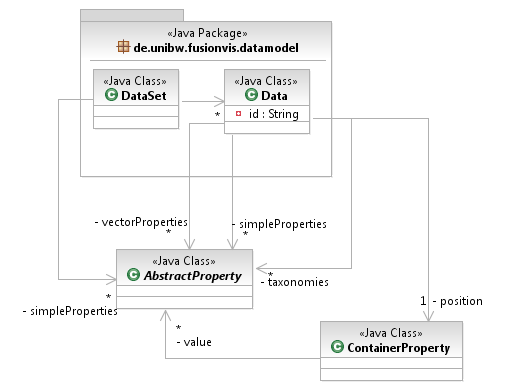
\includegraphics[width=0.75\textwidth]{Bilder/DataModelOverview.png}
	\caption{�bersicht des Datenmodells}
	\label{fig:DataModelOverview}
\end{figure}
	\item[DataSet] Die Klasse \emph{DataSet} kapselt die einzelnen Datens�tze in Form einer Liste. Diese Klasse ist die zentrale Datenstruktur, die f�r alle weiteren Prozesse die notwendigen Informationen bereith�lt. Sie besteht im Wesentlichen aus zwei Bestandteilen. Der erste ist die angesprochene Liste der gespeicherten Daten. Weiterhin kann sie Eigenschaften erfassen, die nicht einem bestimmten Datum zu eigen sind, sondern global f�r die gesamte Datensammlung gelten. Das Benutzen dieser Eigenschaften ist aber fakultativ, um eine hohe Flexibilit�t zu gew�hrleisten.
Die Typisierung der Eigenschaften wird weiter unten dargestellt.

  \item[Data] Die Klasse \emph{Data} kapselt ein einzelnes Datum. Wie bereits in Abschnitt \ref{ch:Eingabedaten} dargelegt, sind die notwendigen Bestandteile eines Datensatzes ein Bezeichner, der innerhalb einer Datensammlung eindeutig sein muss, sowie eine Positionsangabe. Diese ist mithilfe einer zusammengesetzten Eigenschaft festgehalten. Das Eigenschaftssystem wird weiter unten noch detailliert beschrieben.
  
\begin{figure}[hb!]
	\centering
		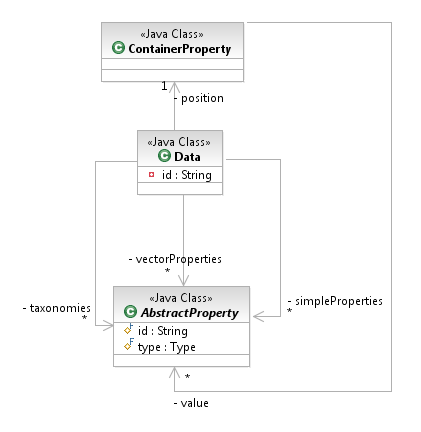
\includegraphics[width=0.5\textwidth]{Bilder/dataModelData.png}
	\caption{Aufbau der Klasse Data}
	\label{fig:dataModelData}
\end{figure}


Zus�tzlich zu diesen beiden obligatorischen Angaben erfasst die Data-Klasse weiterhin drei Listen von Eigenschaften.
\begin{itemize}
	\item einfache Eigenschaften
	\item zusammengesetzte Eigenschaften
	\item Taxonomien
\end{itemize}
Die einfachen Eigenschaften sind in der Lage textuelle und numerische Merkmale eines Datensatzes zu erfassen. Sie sind Grundlage f�r die sp�tere Visualisierung. Die zusammengesetzten Eigenschaften erm�glichen das Ablegen von vektoriellen Gr��en, wie zum Beispiel einer Blickrichtung, Geschwindigkeiten oder Beschleunigungen usw. Auch ist es m�glich, mit ihrer Hilfe baumartig strukturierte Eigenschaften zu erfassen.

Die Taxonomien umfassen eine Liste m�glicher Klassifikationen, die einem Datensatz zu eigen sein k�nnen. Auch ihre Angabe ist nicht zwingend erforderlich.

Der Aufbau einer \emph{Data}-Klasse kann in Abbildung \ref{fig:dataModelData} nachvollzogen werden.
\end{description}
\paragraph{Eigenschaften}
\label{sec:Eigenschaften}
Die Eigenschaften der Datensammlung, wie auch die der Daten an sich, sollten so generisch aufgebaut sein, dass sie f�r m�glichst viele unterschiedliche Anwendungsgebiete ohne �nderung und Anpassung �bernommen werden k�nnen. 

Beim Entwurf fiel auf, dass die auftretenden Eigenschaften nach zwei Kriterien zerfallen. Auf der einen Seite kann nach Dimension der Eigenschaften unterschieden werden. So kann zum Beispiel gespeichert werden, ob die Einheit in einem Gefechtssimulator feindlich, freundlich oder neutral ist. Weiterhin w�re es m�glich, eine Gewichtsangabe zu speichern. In beiden F�llen handelt es sich um eine einfache, weil eindimensionale, Eigenschaft. 

Im Gegensatz dazu gibt es zusammengesetzte Eigenschaften wie vektorielle Gr��en (Ausrichtung, Beschleunigung). In diesen Bereich fallen auch Gliederungsinformationen oder Unterstellungsverh�ltnisse. Eine zusammengesetzte Eigenschaft besteht damit entweder aus einfachen oder wiederum aus zusammengesetzten Eigenschaften.
Diese Unterscheidung f�hrte im Entwurf zur Auswahl des Composite-Patterns (nach \cite{designpatterns}) f�r die Modellierung des Sachverhalts.

Das zweite Kriterium, in das die Informationen der Daten zerfallen, ist ihr Typ. Um einen Kompromiss zwischen einem kompakten Datenmodell und einem breiten Spektrum unterst�tzter Typen zu gew�hrleisten, fiel die Entscheidung auf folgende Datentypen:
\begin{itemize}
	\item Boolean
	\item Char
	\item Date [ANM]
	\item Float
	\item Integer
	\item String
\end{itemize}
Um die grundlegenden Bed�rfnisse zu stillen, h�tte auch die Auswahl eines Flie�kommadatentyps, mit dem sich auch ganze Zahlen darstellen lassen, und ein Zeichenkettendatentyp, mit dem alle anderen Informationen gespeichert werden k�nnen, ausgereicht. Eine noch kleinere Teilmenge, die nur den String-Datentyp umfasst, w�re unter Ausnutzung von programmiersprachenspezifischen Typumwandlungen auch denkbar gewesen. Diese beiden M�glichkeiten wurden aber im Hinblick auf die komfortablere Handhabung verworfen.
\begin{figure}[H]
	\centering
		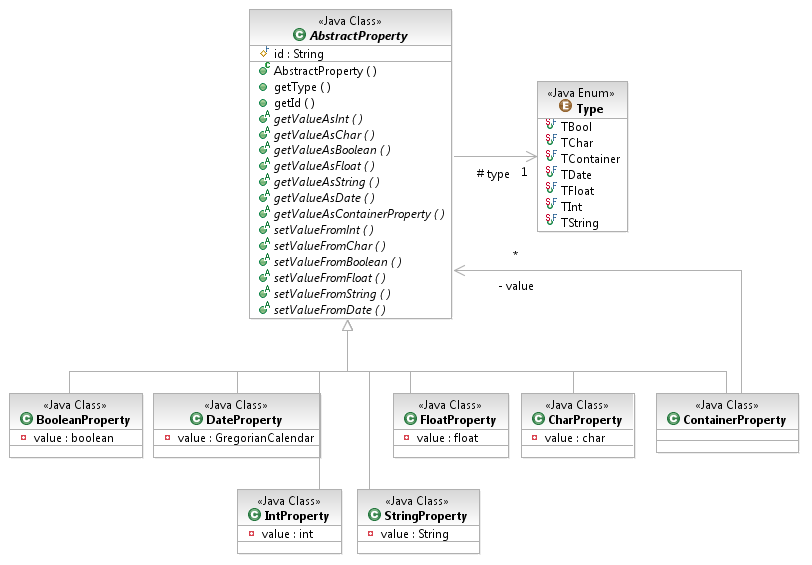
\includegraphics[width=0.75\textwidth]{Bilder/dataModelProperties.png}
	\caption{Eigenschaftssystem im Datenmodell}
	\label{fig:dataModelProperties}
\end{figure}

Der resultierende Entwurf ist in Abbildung \ref{fig:dataModelProperties} dargestellt. Er besteht aus der abstrakten Eigenschaft, den konkreten Implementierungen nach Datentypen und der Zusammengesetzten Eigenschaft.

\begin{description}
	\item[AbstractProperty] Die abstrakte Klasse dient als Muster f�r die konkreten Implementierungen. Sie wird �ber einen Bezeichner eindeutig identifiziert. Es bietet sich hier an, menschenlesbare Namen zu verwenden, die zugleich beschreibenden Charakter haben. Zus�tzlich hat jede Eigenschaft einen Typ. Dieser ist bereits in der abstrakten Klasse implementiert, um zur Laufzeit ohne Kenntnis der genauen Implementierung den jeweiligen Typ der Eigenschaft abfragen zu k�nnen.
	
Der Satz an abstrakten Methoden bildet die notwendige Schnittstelle, um den Wert einer Eigenschaft zu lesen und zu schreiben. Hier stellt sich die Frage, warum eine abstrakte Klasse und nicht etwa ein Interface gew�hlt wurde. Die Antwort ergibt sich aus der M�glichkeit, die Typinformationen und den Bezeichner in der allgemeinen Eigenschaft vorhalten zu k�nnen. Das entlastet den Programmierer bei der Umsetzung der konkreten Implementierungen, da er sich darum nicht mehr k�mmern muss.

Aus Sicht des Composite-Patterns stellt \emph{AbstractProperty} die Component-Klasse dar.
\item[Typ-Property] Die Implementierungen der abstrakten Klasse tragen in der Umsetzung die Verantwortung, einen zum Typ passenden Wert zu speichern. Dieser wird in der Ausgestaltung der Manipulationsmethoden gesetzt und gelesen. Wo notwendig sind Typumwandlungen durchzuf�hren, unsinnige Umwandlungen (zum Beispiel das Konvertieren eines bool'schen Datentyps in ein Datum) mit einer Ausnahmebehandlung quitiert werden.

Eine Typ-Property ist die im Composite-Pattern als \emph{Leaf} bezeichnete Klasse.
\item[ContainerProperty] Die zusammengesetzte Eigenschaft verwaltet ihre zugeh�rigen Eigenschaften in einer Liste von \emph{AbstractProperty}-Klassen. Sie kann aus diesem Grund aus Typ-Property-Klassen bestehen oder wiederum aus zusammengesetzten Eigenschaften. \emph{ContainerProperty} stellt im Pattern den Composite dar.
\end{description}
\paragraph{Erweiterbarkeit}
Das Datenmodell ist an der Stelle der Eigenschaften erweiterbar. Um einen neuen Typ einzuf�hren m�ssen vier Schritte durchgef�hrt werden: 

In der Enumeration der Typen ist der neue einzuf�hren. Weiterhin m�ssen in der \emph{AbstractProperty} die Zugriffs- und Manipulationsmethoden f�r den neuen Typ abstrakt definiert werden. Daraus folgt, dass bestehende Typen diese Methoden implementieren m�ssen. Macht eine Typumwandlung Sinn, dann kann diese umgesetzt werden. Wenn sie unsinnig sind, dann wendet man Ausnahmenbehandlung an.

Abschlie�end muss nun eine neue Typ-Property Klasse erstellt und implementiert werden, die von ihrem abstrakten Vorbild erbt. 
Durch diese vier Schritte hat man somit das Datenmodell um einen Typ erweitert.
\subsection{�bersicht �ber das Frontend des Frameworks}
\label{ch:Framework}
\begin{figure}[ht!]
	\centering
		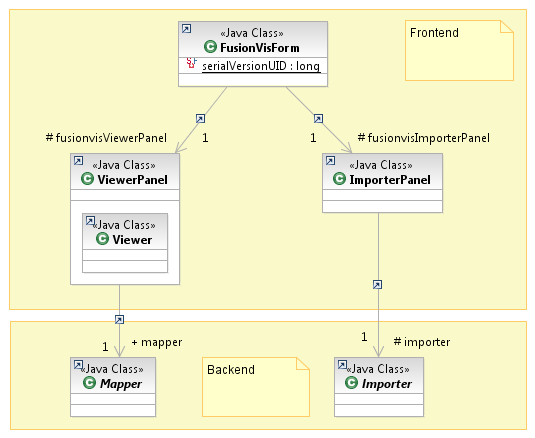
\includegraphics[width=0.75\textwidth]{Bilder/framework.png}
	\caption{�bersicht des Frameworks (Frontend/Backend)}
	\label{fig:framework}
\end{figure}

Das erstellte Framework besteht im Wesentlichen aus zwei Teilen. Auf der einen Seite stehen die f�r den Benutzer sichtbaren Klassen, an denen nicht notwendigerweise eine Anpassung vorgenommen werden muss, um ein lauff�higes Programm zu erstellen. Zu diesen Klassen geh�rt auf oberster Ebene die Klasse \emph{FusionVisForm}. Das ist die dem Benutzer angezeigte Programmoberfl�che. Sie besteht aus einem Men� mit implementierter Funktion zum Ausw�hlen von XML-Dateien und zum Schlie�en des Programms. 

Die Benutzeroberfl�che enth�lt weiterhin zwei \emph{JPanel}-Klassen, die es dem Benutzer erm�glichen, eine textuelle und eine visuelle Darstellung der Daten zu sehen. 
\begin{description}
	\item[ImporterPanel] F�r die textuelle Sicht ist das \emph{ImporterPanel} vorgesehen. Es bietet die M�glichkeit, die Daten nach bestimmten Eigenschaften zu filtern und diese mit ihren Eigenschaften in Textform anzuzeigen. Das Model, auf dem gearbeitet wird, ist das in Abschnitt \ref{ch:Datenmodell} beschriebene Datenmodell. Somit ist das ImporterPanel auch v�llig unabh�ngig von dem genauen Inhalt der Daten, solange diese in das beschriebene Model �berf�hrt wurden. Daf�r ist der Importer zust�ndig, der im n�chsten Abschnitt beschrieben wird.

	\item[ViewerPanel]Die zweite \emph{JPanel}-Klasse ist das \emph{ViewerPanel}. Es ist verantwortlich f�r die dreidimensionale Anzeige der Daten. Dazu ist es notwendig, das vorhandene Datenmodell in die Struktur eines Szenenbaums zu �berf�hren. Der Szenenbaum wird in Abschnitt \ref{sec:Szenenbaum} beschrieben. Dieser Schritt wird vom \emph{Mapper} bewerkstelligt, der im n�chsten Abschnitt erkl�rt wird.

Der erstellte Szenenbaum kann nun von einem Viewer angezeigt werden. Dieser beinhaltet eine OpenGL-Anzeigefl�che, welche die dreidimensionale Darstellung �bernimmt und es dem Benutzer erlaubt, sich in den visualisierten Daten zu bewegen, Datens�tze mittels Mousepickings (siehe Abschnitt \ref{ch:mousepicking}) auszuw�hlen und diese somit im \emph{ImporterPanel} zu inspizieren. Auch der umgekehrte Weg ist m�glich, also das Ausw�hlen eines Datums in der textuellen Ansicht, was eine Hervorhebung seiner Visualisierung im ViewerPanel zur Folge hat.
\end{description}

Zusammenfassend kann man zum Frontend des Frameworks sagen, dass die von den konkreten XML-Daten unabh�ngigen Funktionen bereits implementiert sind. Der Anwender muss lediglich festlegen, was wie dargestellt werden soll. Das \emph{Was} ist der Prozess des �berf�hrens von XML in das Datenmodell des Frameworks und wird im \emph{Importer} festgeschrieben. Das \emph{Wie} ist die Frage nach der Art und Weise, wie die Daten dreidimensional dargestellt werden sollen und wird im \emph{Mapper} beantwortet.

\subsection{�bersicht �ber das Backend des Frameworks}
Das Backend besteht im Wesentlichen aus den zwei oben erw�hnten Komponenten \emph{Importer} und \emph{Mapper}. Im Folgenden soll die Funktion der beiden erl�utert und notwendige Schritte der Spezialisierung beschrieben werden.

Die Spezialisierung bezieht sich auf das Implementieren abstrakter Methoden, die in den beiden als abstrakt gekennzeichneten Klassen die eigentliche Funktion enthalten sollen.
\subsubsection{Importer}
Der \emph{Importer} ist, wie bereits im vorherigen Abschnitt angemerkt, daf�r verantwortlich, die Daten aus einer XML-Datei zu lesen. An die Struktur muss eine Voraussetzung gemacht werden, um den Import automatisiert durchf�hren zu k�nnen: Die Datens�tze m�ssen als Elemente des ersten Elements unter dem Wurzelknoten in der XML-Dateien stehen. Ein Beispiel f�r eine XML-Datei, die diese Anforderung erf�llt, ist in Listing \ref{code:xmlexample} aufgef�hrt.

Ist die Voraussetzung erf�llt, liest der \emph{Importer} die XML-Datei aus und extrahiert die DOM-Knoten der Datenelemente. Die Wahl des DOM-Parsers f�r diese Aufgabe wird noch in Abschnitt \ref{sec:DOMParser} genauer erl�utert. 

\lstset{%
language=XML,
basicstyle={\ttfamily,\footnotesize},
numbers=left,                   % where to put the line-numbers
numberstyle=\footnotesize,      % the size of the fonts that are used for the line-numbers
stepnumber=2,
}%
\begin{lstlisting}[breaklines=true,frame=tlRB,captionpos=b,caption={Beispiel f�r eine wohlgeformte XML-Datei},label=code:xmlexample]
<Situation>
  <Units>
   <Unit>
      <Name>FriendlyTank1</Name>
      <Location>
        <Lat>52.796629714678467</Lat>
        <Lon>9.89990561649954</Lon>
        <LastModified>2009-02-20T10:25:36+01:00</LastModified>
      </Location>
    </Unit>
    <Unit>
      <Name>FriendlyTank2</Name>
      <Location>
        <Lat>52.794038961891268</Lat>
        <Lon>9.9011727699025922</Lon>
        <LastModified>2009-02-20T10:25:36+01:00</LastModified>
      </Location>
    </Unit>
  </Units>
</Situation>
\end{lstlisting}

Der \emph{Importer} h�lt bereits notwendige Datenstrukturen vor. Zum einen sind dies zwei Membervariablen (\emph{id}, \emph{position}). Diese dienen dem Speichern der XML-Elementnamen, die den Wert f�r Position und Bezeichner eines Datums liefern. �hnlich gibt es drei Listen, die die Elementnamen enthalten, die als einfache, zusammengesetzte Eigenschaften oder als Taxonomie extrahiert werden.

\paragraph{Spezialisierung}
\label{sec:ImporterSpezialisierung}
Zur  Spezialisierung eines \emph{Importers} f�r ein bestimmtes Datenformat m�ssen zwei Schritte durchlaufen werden.  Als erstes sollten die in das Datenmodell als Eigenschaft von Daten zu �bernehmenden XML-Elemente auf die oben angesprochenen Membervariablen und Listen verteilt werden. 

Als n�chstes muss nun die Methode \emph{extractDataFromNode()} implementiert werden. Ihr wird ein Knoten des DOM-Dokumentbaums �bergeben. Dieser zeigt auf ein Element, dass als Datum in das Datenmodell �bernommen werden soll. Die Aufgabe der Funktion ist es nun, nach den Vorstellungen des Anwenders ein Data-Objekt zu instanzieren, das die in den vorher spezifizierten Listen stehenden Eigenschaften enth�lt.

\paragraph{Hilfsfunktionen}
\label{sec:ImporterHilfsfunktionen}
In der \emph{Importer}-Klasse sind bereits zwei Hilfsfunktionen implementiert, die dem Anwender die Arbeit beim erzeugen der Data-Objekte vereinfachen sollen. Die Methode \emph{parseDate()} dient dem Auslesen eines Datums aus einem String. F�r die genauere Dokumentation sei hier auf das JavaDoc verwiesen.

Die Methode  \emph{extractSimpleProperty(Node, Type)} erzeugt eine einfache Eigenschaft (siehe \ref{sec:Eigenschaften}) eines angegebenen Typs aus einem DOM-Knoten. Um beispielsweise in Zeile 4 von Listing \ref{code:xmlexample} eine Eigenschaft \emph{Name} als String zu extrahieren, muss die Hilfsfunktion lediglich mit der Node aufgerufen werden, die auf dieses Element zeigt. Zus�tzlich wird der gew�nschte Typ (hier: \emph{Type.TString}) �bergeben.


\lstset{%
language=Java,
showstringspaces=false,
keywordstyle=\color{red},
breaklines=true,
frame=single
commentstyle=\color{blue},
stringstyle=\color{green},
backgroundcolor=\color{white},
basicstyle={\ttfamily,\footnotesize},       % the size of the fonts that are used for the code
numbers=left,                   % where to put the line-numbers
numberstyle=\footnotesize,      % the size of the fonts that are used for the line-numbers
stepnumber=2
}%
\begin{lstlisting}[breaklines=true,frame=tlRB,captionpos=b,caption={Beispielhafte Implementierung der \emph{extractDataFromNode()}-Methode}, ,label=code:extractDataFromNode]
  protected Data extractDataFromNode(Node unitNode) throws Exception {
    Data result = null;
    NodeList list = unitNode.getChildNodes();
    // Erster Durchlauf zum Finden des Bezeichners
    for (int i = 0; i < list.getLength(); i++) {
      if (list.item(i).getNodeType() != Node.ELEMENT_NODE)
        continue; // wenn kein Element, dann skip
      Node element = list.item(i);
      if (element.getNodeName().equals(id))
        result = new Data(element.getTextContent());
    }
    // Zweiter Durchlauf f�r das setzen der restlichen Eigenschaften
    for (int i = 0; i < list.getLength(); i++) {
      if (list.item(i).getNodeType() != Node.ELEMENT_NODE)
        continue; // wenn kein Element, dann skip
      Node element = list.item(i);
      // Position setzen
      if (element.getNodeName().equals(position))
        result
            .setPosition(extractContainerProperty(element,
                "Position"));
      else if (simplePropertyList.contains(element.getNodeName()))
        if (element.getNodeName().equals("IsPlatform"))
          result.addAbstractProperty(extractSimpleProperty(element,
              Type.TBool));
        else
          result.addAbstractProperty(extractSimpleProperty(element,
              Type.TString));
      else if (vectorPropertyList.contains(element.getNodeName()))
        result.addContainerProperty(extractContainerProperty(element,
            element.getNodeName()));
      else if (taxonomyList.contains(element.getNodeName()))
        result.addTaxonomie((extractSimpleProperty(element)));
      else ; // skip
    }
    return result;
  }
 \end{lstlisting}
%\paragraph{Anbindung an XML}
%\paragraph{Instanzieren des Datenmodells}
\subsubsection{Mapper}
Bereits im vorletzten Abschnitt wurde angesprochen, dass der \emph{Mapper} daf�r Sorge tr�gt, dass das Datenmodell in eine dreidimensionale Darstellung �berf�hrt wird. Da nicht f�r jedes Problem auch dieselbe Visualisierung zielf�hrend ist, besteht hier die M�glichkeit zur Individualisierung.

Bei der konkreten Implementierung sind zwei unterschiedliche Aspekte zu unterscheiden: Auf der einen Seite ist die Frage, wie die Daten an sich dargestellt werden, zum Beispiel in Bezug auf Form und Farbe und das sonstige Erscheinungsbild. Auf der anderen Seite muss spezifiziert werden, in welcher Art und Weise die Dimensionen der Daten dargestellt werden.

Resultat des Mappingvorgangs soll ein Szenenbaum sein. Er ist die f�r die Grafikengine lesbare Form des Datenmodells. Dieser Szenenbaum muss bei jeder Ver�nderung des Datenmodells aktualisiert werden. Als solche z�hlt zum Beispiel das Filtern von Daten nach bestimmten Eigenschaften oder das Erstellen einer Sicht auf das Datenmodell.
\paragraph{Spezialisierung}
\label{sec:MapperSpezialisierung}
Wie oben bereits beschrieben hat die Spezialisierung im \emph{Mapper} zwei Aspekte. Auf der einen Seite kann die Gestalt eines einzelnen Datums spezifiziert werden und auf der anderen Seite die Position dieses Datums im dreidimensionalen Raum. Eine vollst�ndige Trennung ist in der derzeitigen Version nicht gelungen. Inwiefern sich das auswirkt, wird im Folgenden gezeigt.

\subparagraph{Position und Projektion}
\label{sec:PositionUndProjektion}
Eine grundlegende Entscheidung bei der Visualisierung von Daten ist, wie aus den Rohdaten eines Datums die Koordinaten im dreidimensionalen Raum gewonnen werden k�nnen. Bereits in Abschnitt \ref{ch:Eingabedaten} wurde beschrieben, dass solche Rohdaten existieren m�ssen. Ebenfalls ist darauf verwiesen worden, dass ungeeignete Rohdaten (weder in Gleitkomma-, noch in ganzzahliger Darstellung) an dieser Stelle durch einen geeigneten Homomorphismus umzuwandeln sind.

Der erste Schritt zur Individualisierung des \emph{Mappers} ist die Bestimmung der Ausma�e der Projektionsfl�che. Dieser Begriff meint die Ebene, die trivialisiert durch L�nge und Breite aufgespannt wird. Ihre Festlegung erfolgt durch die Implementierung der \emph{getSize()}-Methode. Hier gibt es zwei Varianten der Umsetzung. Es kann eine feste, von den Daten unabh�ngige Projektionsfl�che gew�hlt werden. Eine ma�stabsgetreue Abbildung entf�llt somit. Vorteil dieser Art ist, dass bereits zur Implementierungszeit absch�tzbar ist, wie gro� die maximalen Entfernungen ausfallen. Somit k�nnen Entscheidungen, wie die Positionierung der Kamera [REF], sinnvoll getroffen werden.\\
Eine andere M�glichkeit ist eine von den Eingabedaten abh�ngige Projektionsfl�che. Hier entf�llt das absch�tzbare Ausma� der Darstellung zum Wohle der ma�stabsgetreuen Abbildung.\\
Eine der wichtigsten Verwendungen dieser Methode liegt im sp�teren Erzeugen des Gittermusters, welches eine bessere Einsch�tzung der Dimensionen erm�glicht.

Der zweite Schritt zur Individualisierung ist die Festlegung der Skalierung der Position auf den einzelnen Dimensionen. Die Notwendigkeit hierf�r kann sich aus ung�nstig gestalteten Rohdaten ergeben. Um zum Beispiel Zeiten in Ortsangaben umzuwandeln, kann man auf die interne Darstellung eines Zeitpunktes in die Zahl der Millisekunden seit dem 01.01.1970 zur�ckgreifen. Hieraus ergeben sich jedoch schon f�r kurze Zeitspannen riesige Zahlenwerte, die zu ebensogro�en Ausma�en der Darstellung f�hren w�rden.\\
Mit der Implementierung der Methode \emph{getDimensionFactors()} kann diesem Umstand Rechnung getragen werden. Ist eine Skalierung nicht notwendig, so kann die triviale Skalierung mit dem Faktor 1 erfolgen.

Der letzte Schritt zur Positionierung ist die Festlegung eines Datums auf eine genaue Koordinate in der dreidimensionalen Darstellung. Implementiert werden muss dies gleichzeitig mit der Festlegung der Gestalt eines Datensatzes. Wie dies zu erfolgen hat, ist in der allgemeinen Beschreibung zur Positionierung in Abschnitt [REF jme, Positionierung] beschrieben. Der Ort dieser Implementierung ist die im Folgenden beschriebene Methode. 

\subparagraph{Gestalt}
\label{sec:Gestalt}
Die Gestalt eines Datums wird von der Methode \emph{extractNodeFromData()} bestimmt. Sie hat die Aufgabe, einen Szenenknoten (siehe Abschnitt [REF]) f�r jeden Datensatz zu erstellen. Bestandteil muss auf jeden Fall ein Grafikobjekt, wie in Abschnitt [REF, Visualisierung eines Datums] beschrieben, sein.  Im letzen Abschnitt wurde bereits angesprochen, dass ebenfalls die Festlegung der Koordinate des Grafikobjekts an dieser Stelle zu erfolgen hat. \\
In dieser Methode kann der Benutzer neben Form, Gr��e, Position und sonstigen Eigenschaften, wie zum Beispiel Renderingoptionen (siehe Abschnitt \ref{sec:Transparenz}), auch die Texturierung von Objekten festlegen. Es ist jedoch nicht immer zweckm��ig, f�r jedes Objekt eine individuelle Textur zuzuweisen. Aus diesem Grund gibt es eine weitere Methode, die es gilt zu implementieren.

Die Methode \emph{texture()} hat zur Aufgabe die Grafikobjekte eines �bergebenen Szeneknotens zu texturieren. Dies kann anhand von bestimmten Eigenschaften geschehen. Enumerationen eignen sich hierbei sehr gut. Wie in Abschnitt \ref{ch:visualisierungDatum} beschrieben, sollte man sich an dieser Stelle auf eine noch vom Kurzzeitged�chtnis erfassbare Menge an Farben beschr�nken. Ist es jedoch nicht notwendig, so kann die Implementierung dieser Methode leer verbleiben.
\paragraph{Hilfsfunktionen}
\label{sec:MapperHilfsfunktionen}
Hilfsfunktionen der Art, wie sie aus dem \emph{Importer} bekannt sind, gibt es im \emph{Mapper} nicht. An dieser Stelle soll jedoch die Methode \emph{getDataRoot()} erw�hnt werden, die den Zugriff auf den vom \emph{Mapper} erstellten Szenegraphen erm�glicht. Sie ist in zwei Auspr�gungen vorhanden: Einerseits ohne Angabe von Argumenten um an die Visualisierung des Datenmodells zu gelangen, das bei der Erstellung des \emph{Mappers} �bergeben wurde. Andererseits kann auch ein Datenmodell, welches zum Beispiel durch Filtern entstanden ist, �bergeben werden. Es wird automatisch zum neuen Modell des \emph{Mappers} und daraus wird der neue Szenengraph erzeugt.


\subsection{Zusammenspiel der Komponenten}
Nachdem im letzten Abschnitt die notwendigen M�glichkeiten zur Individualisierung durch konkrete Implementierung erl�utert wurden, soll im Folgenden das Zusammenspiel der Komponenten und damit die Funktionsweise des Frameworks anhand von ausgew�hlten Aspekten skizziert werden. 
\subsubsection{Visualisierungsprozess}
\begin{figure}[htb]
	\centering
		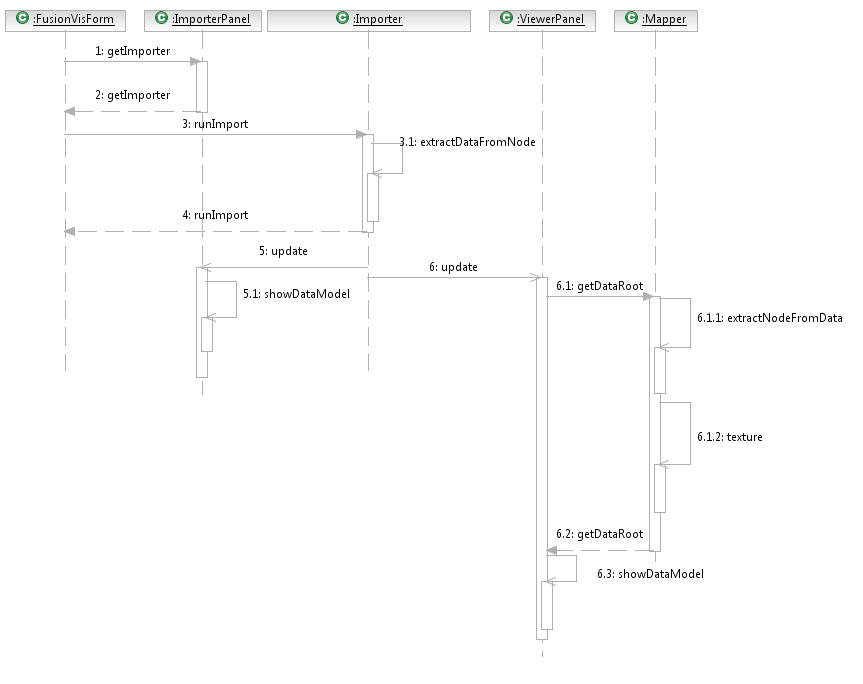
\includegraphics[width=0.90\textwidth]{Bilder/VisualisierungsProzess.png}
	\caption{Ablauf des Visualisierungsprozesses}
	\label{fig:VisualisierungsProzess}
\end{figure}

Ein wesentlicher Punkt in der Interaktion der Komponenten ist der Visualisierungsprozess, der alle Komponenten des Frontends und des Backends erfasst. Hier die dazugeh�rige chronologische Abfolge:

\begin{enumerate}
	\item Der Benutzer w�hlt eine XML-Datei aus. Die Benutzeroberfl�che ruft daraufhin vom zu ihr geh�renden \emph{ImporterPanel} den \emph{Importer} ab.

	\item Das \emph{ImporterPanel} liefert den geforderten \emph{Importer}.

	\item Die Form st��t nun den eigentlichen Importvorgang im \emph{Importer} an. Der \emph{Importer} greift dabei auf die vom Benutzer implementierte  \emph{extractDataFormNode()}-Methode zur�ck.

	\item Nach dem Ansto�en hat die Form nichts mehr mit dem restlichen Vorgang zu tun.

	\item Aufgrund der Ver�nderung des Datenmodells durch das Laden von Daten m�ssen die Sichten in den Panels aktualisiert werden. Auf der einen Seite aktualisiert das \emph{ImporterPanel} die textuelle Darstellung der Daten. 

	\item Auf der anderen Seite muss das \emph{ViewerPanel} die grafische Datensicht aktualisieren.

\begin{enumerate}
	\item Dazu muss das Datenmodell in einen Szenenbaum umgewandelt werden. Diese Aufgabe delegiert das Panel an den \emph{Mapper}. Dieser erstellt mithilfe der aus dem letzten Abschnitt bekannten Methode \emph{extractNodeFromData()} den Baum. Mit der Methode \emph{texture()} werden die Visualisierungen der Daten anschlie�end eingef�rbt.

	\item Den fertigen Szenenbaum gibt der \emph{Mapper} an das \emph{ViewerPanel} zur�ck.

	\item Abschlie�end stellt das \emph{ViewerPanel} die Daten grafisch dar.
\end{enumerate}
\end{enumerate}

Der beschriebene Prozess kann in Abbildung \ref{fig:VisualisierungsProzess} nachvollzogen werden.

Die angesprochene Aktualisierung der beiden unterschiedlichen Darstellungen erfolgt durch die Anwendung des Observer-Patterns (nach \cite{ designpatterns}). Dabei tr�gt die Form die Verantwortung, dass auch beide Panels beim Importer als Observer registriert werden. Diese Funktion ist aber bereits in der FusionVisForm implementiert, sodass der Benutzer von dieser Aufgabe unbehelligt bleibt.  
\subsubsection{ImporterPanel und ViewerPanel}
Bereits im letzten Abschnitt ist deutlich geworden, dass bei �nderungen am Datenmodell zwangsl�ufig die Sichten aktualisiert werden m�ssen. Eine Situation, bei der diese Aktion notwendig ist, ist der Datenimport. Im Folgenden werde ich die beiden weiteren Aktivit�ten beschreiben, bei denen sich die Panels abstimmen m�ssen.

\paragraph{Filtern des Datenmodels}
\label{sec:FilternDesDatenmodels}
�ber das \emph{ImporterPanel} ist es m�glich, die Sicht auf das Datenmodell zu beschr�nken, indem Datens�tze anhand von nicht vorhandenen Eigenschaften ausgeblendet werden. Wie dies aussieht, ist in Abschnitt \ref{ch:Prototyp} beschrieben.

Das Ver�ndern des Datenmodells durch Ausgrenzen bestimmter Datens�tze macht die Aktualisierung der Sicht im \emph{ViewerPanel} notwendig. Dies geschieht auf die gleiche Art und Weise wie ein Neuimport von Daten, denn prinzipiell ist das Filtern von Daten nur die Gegenoperation zum Import und somit nur eine Ver�nderung am Datenmodell. Aus diesem Grund wird auch an dieser Stelle das Observerpattern genutzt. 

Problematisch ist hierbei, dass die beiden Panels bereits eine Oberklasse haben und somit nicht von der in Java bereits zur Verf�gung gestellten Observerklasse erben k�nnen. Ein Ausweg aus diesem Problem wird in Abschnitt \ref{sec:ObserverPatternBeiAbgeleitetenKlassen} dargestellt.

\paragraph{Selektion von Datens�tzen}
\label{sec:SelektionVonDatensaetzen}
Eine weitere Aktivit�t, in der die beiden Panels kooperieren m�ssen, ist die Selektion eines Datensatzes. Ein Datum kann entweder im \emph{ImporterPanel}, in der textuellen, oder im \emph{ViewerPanel}, in der grafischen Darstellung, ausgew�hlt werden.

Ziel soll es sein, dass ein Datum, das in der einen Sicht ausgew�hlt wird, auch in der andern Sicht als selektiert erscheint. Die Auswahl an sich ist im \emph{ImporterPanel} aufgrund der Bordmittel von Swing [REF Technologie, Java, SWING] trivial. Im \emph{ViewerPanel} wird dies um einiges schwieriger, weil es sich dabei um einen sogenannten Mousepick handelt. Problematisch ist dabei, dass auf der zweidimensionalen Fl�che des Bildschirms ein Objekt im dreidimensionalen Raum ausgew�hlt werden soll. F�r die L�sung des Problems sei auf Abschnitt \ref{ch:mousepicking} verwiesen.

Nachdem ein Datensatz ausgew�hlt wurde, wird auch an dieser Stelle wieder mit Hilfe des Observer-Patterns das jeweils andere Panel �ber das Ereignis informiert, sucht in seiner Darstellung den selektierten Datensatz und hebt ihn hervor.

Die Kopplung der beiden Datenbest�nde erfolgt �ber den Bezeichner des Datums. Bereits in Abschnitt \ref{sec:Identifizierbarkeit} wurde gefordert, dass es sich hierbei um eine eindeutige Eigenschaft handeln muss. W�re dies nicht der Fall, ist das geforderte Ziel der abgestimmten Auswahl schlicht nicht zu erreichen. 

\subsubsection{ViewerPanel und Viewer}
Aus der Abbildung \ref{fig:framework} wird deutlich, dass der Viewer aus dem allgemeinen Rahmen der Struktur heraus f�llt, da er als innere Klasse des ViewerPanels umgesetzt ist. Dies ist ein aus entwurfs�sthetischen Gesichtspunkten unsch�ner Sachverhalt. \\
Betrachtet man jedoch die enge Zusammenarbeit zwischen dem Panel und dem Viewer, wird klar, warum die pragmatische zugunsten der �sthetischen L�sung gew�hlt wurde. 

Zum Einen sollte das Panel in Hinblick auf Erweiterbarkeit, wie zum Beispiel einstellbare Kameraperspektiven, eine Schnittstelle zum \emph{Viewer} bieten. W�re dieser als separate Klasse umgesetzt,  h�tten viele Methoden und Instanzvariablen publik gemacht werden m�ssen. Eine geeignete Kapselung wird so unm�glich. Aus diesem Grund bietet es sich an, den \emph{Viewer} zwecks der Abschirmung in  das Panel einzubinden.

Ein anderer Aspekt, bei dem genau derselbe Zwiespalt auftritt, ist das Ausw�hlen von Daten im \emph{ViewerPanel}. Da der Aufbau von Komponenten in Swing hierarchisch organisiert ist, klickt der Benutzer beim Selektieren eines Objekts in der dreidimensionalen Darstellung nicht auf die vom Viewer bereitgestellte Zeichenfl�che, sondern in die Form, die wiederum nativ das Ereignis an das zust�ndige Panel weitergibt.

An dieser Stelle bricht jedoch die Kette, denn der \emph{Viewer} ist nicht in die Swing- Klassenstruktur eingebettet. Aus diesem Grunde k�mmert sich das ViewerPanel um die f�r das Ausw�hlen notwendigen Schritte. Zu diesem Zweck ben�tigt es, �hnlich wie oben angesprochen, einen weitreichenden Zugriff auf den \emph{Viewer}. Ohne ihn komplett �ffentlich zu gestalten, f�hrt auch hier der Weg an einer inneren Klasse nicht vorbei.

Aus Sicht der Unterscheidung Framework-Komponenten in Frontend und Backend ist die Zuordnung des Viewers in das Panel vertretbar, denn er ist mit seiner Zeichenfl�che im Gegensatz zum Importer eine sichtbare Komponente.
\section{Visualisierung einer milit�rischen Lage}
\label{ch:Prototyp}
\begin{figure}[htb!]
	\centering
		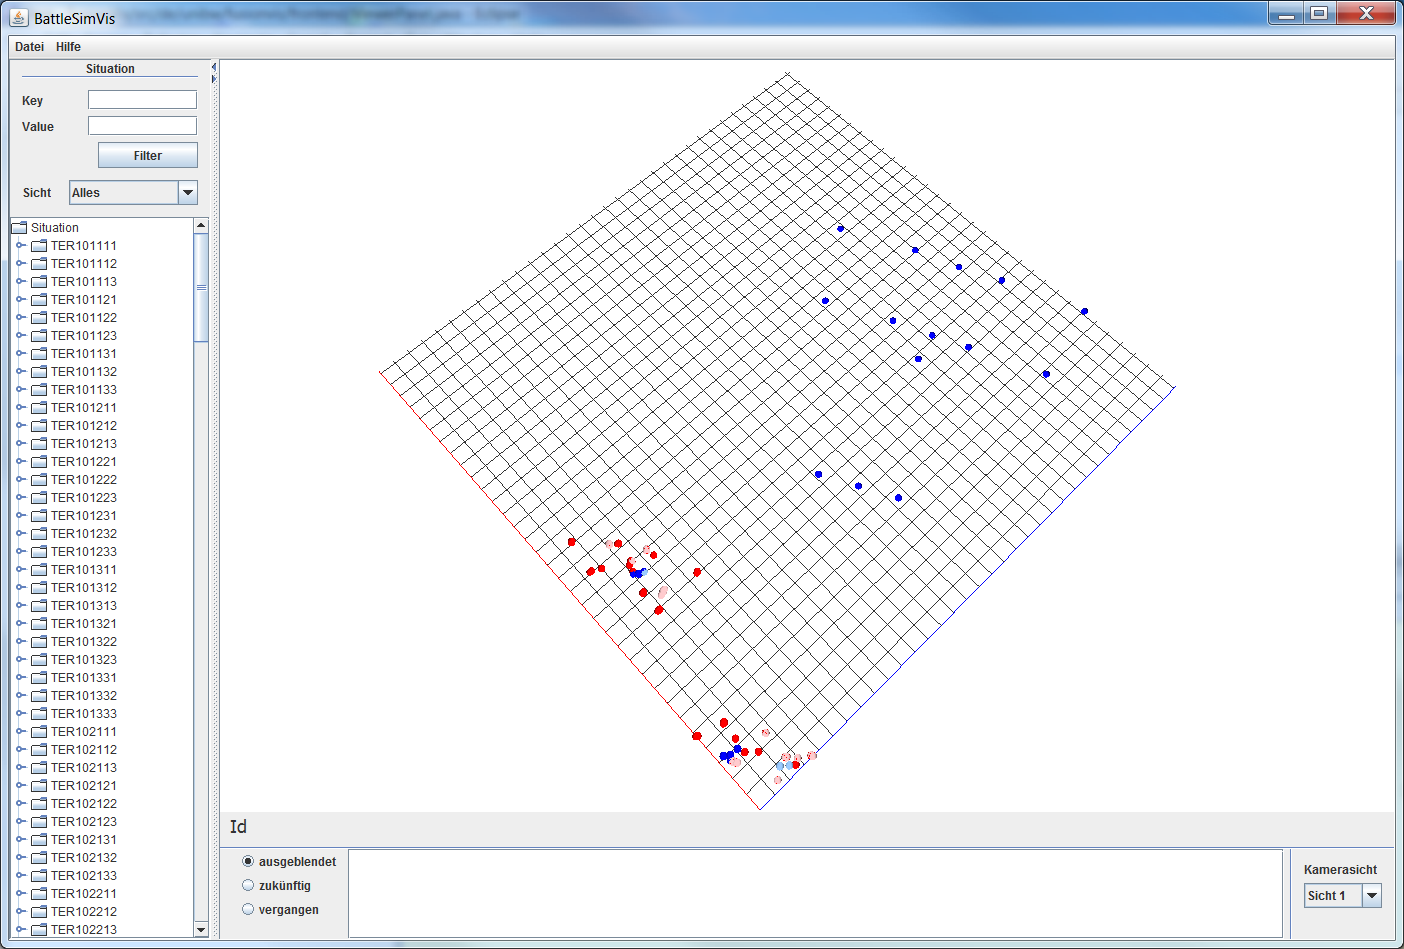
\includegraphics[width=1\textwidth]{Bilder/screen.png}
	\caption{Darstellung einer Lage mit zwei aufeinandertreffenden Bataillonen, insgesamt 251 Datens�tze}
	\label{fig:screen}
\end{figure}


Bereits in Abschnitt \ref{motivation}  wurde die Lage des S2-Offiziers angesprochen, der von den Panzern seines Bataillons Positions- und Feindmeldungen bekommt. Dies geschieht aus Gr�nden der Daten�bertragung in textueller, beschr�nkt menschenlesbarer Form.

\subsection{Problemdarstellung}
\label{sec:Problemdarstellung}

Die Aufgabe des S2-Offiziers ist es, aus diesen Daten ein Lagebild zu erstellen, also die Daten zu visualisieren. Problematisch sind hierbei vor allem die Feindmeldungen. Folgende Lage veranschaulicht das Problem:

In der Norddeutschen Tiefebene treffen zwei eigene Panzer auf zwei gegnerische. Die eigenen Einheiten bewegen sich nicht, sie stehen in teilgedeckter Stellung. Die feindlichen Einheiten bewegen sich mit hoher Geschwindigkeit, eine in Richtung auf die beiden blauen\footnote{Im Kontext von milit�rischen Lagen spricht man von blauen und roten Einheiten. Rot steht hierbei f�r feindliche, blau f�r eigene oder verb�ndete Einheiten.} Panzer, die andere in Querfahrt von Rechts nach Links aus Sicht der beobachtenden Einheiten.

Im Abstand von 60 Sekunden geben die beiden eigenen Panzer drei Mal nacheinander Meldungen �ber die gesichteten Feinde ab.  Daraus resultieren zw�lf Feindmeldungen.

F�r den Offizier, der nun die Daten erh�lt, stellen sich potentiell zw�lf Feindeinheiten dar. Von der Anzahl erg�be das die St�rke einer Kompanie. Dies entspricht nicht der Wirklichkeit. Das Problem, das es nun zu l�sen gilt, ist durch geeignete Visualisierung aus der vermeintlichen Kompanie wieder die zwei eigentlichen Feindpanzer erkennen zu k�nnen.

\subsection{L�sungsansatz}
\label{sec:Loesungsansatz}

Die zahlenm��ige Explosion der potentiellen Feindmeldungen kann durch zwei Ans�tze reduziert werden: 

\subsubsection{Ortsgleichheit}
\label{sec:Ortsgleichheit}

Als erstes gilt es, dass alle Meldungen, die zur selben Zeit gemacht wurden, auf die Lage des gemeldeten Objekts �berpr�ft werden. Wurde an einem Ort (mit einer gewissen Toleranz)  gleichzeitig mehrere Einheiten gemeldet, so kann das daher kommen, dass diese eben von mehreren eigenen Panzern gleichzeitig gesehen wurden.

Mit diesem Ansatz k�nnen die zw�lf Meldungen auf nur noch vermeintlich sechs Feindeinheiten reduziert werden.

\subsubsection{Reichweitenberechnung}
\label{sec:Reichweitenberechnung}

Der n�chste Schritt ist die Analyse der Meldungen, die zu unterschiedlichen Zeiten abgegeben wurden. Unter Annahme der maximalen Geschwindigkeit kann man n�mlich feststellen, ob zwei Meldungen definitiv von unterschiedlichen Feindeinheiten ausgel�st wurden, oder ob die M�glichkeit besteht, dass es sich um ein und dasselbe Objekt handelt.

Gegeben seien daf�r zwei Meldungen. Aus ihnen lassen sich die Zeitdifferenz und die r�umliche Entfernung der beiden voneinander bestimmen. Ist ihre Entfernung gr��er, als die Distanz, die in der errechneten Zeit, unter Annahme der H�chstgeschwindigkeit, h�tte zur�ckgelegt werden k�nnen, so handelt es sich definitiv um unterschiedliche Einheiten.

Auf diese Art und Weise kann die Zahl der potentiellen Einheiten weiter der Zahl der echten Einheiten angen�hert werden und ein aussagekr�ftigeres Lagebild entsteht.

\subsection{Umsetzung mithilfe des Visualisierungsframeworks}
\label{sec:UmsetzungMithilfeDesVisualisierungsframeworks}
\begin{figure}[htb]
	\centering
		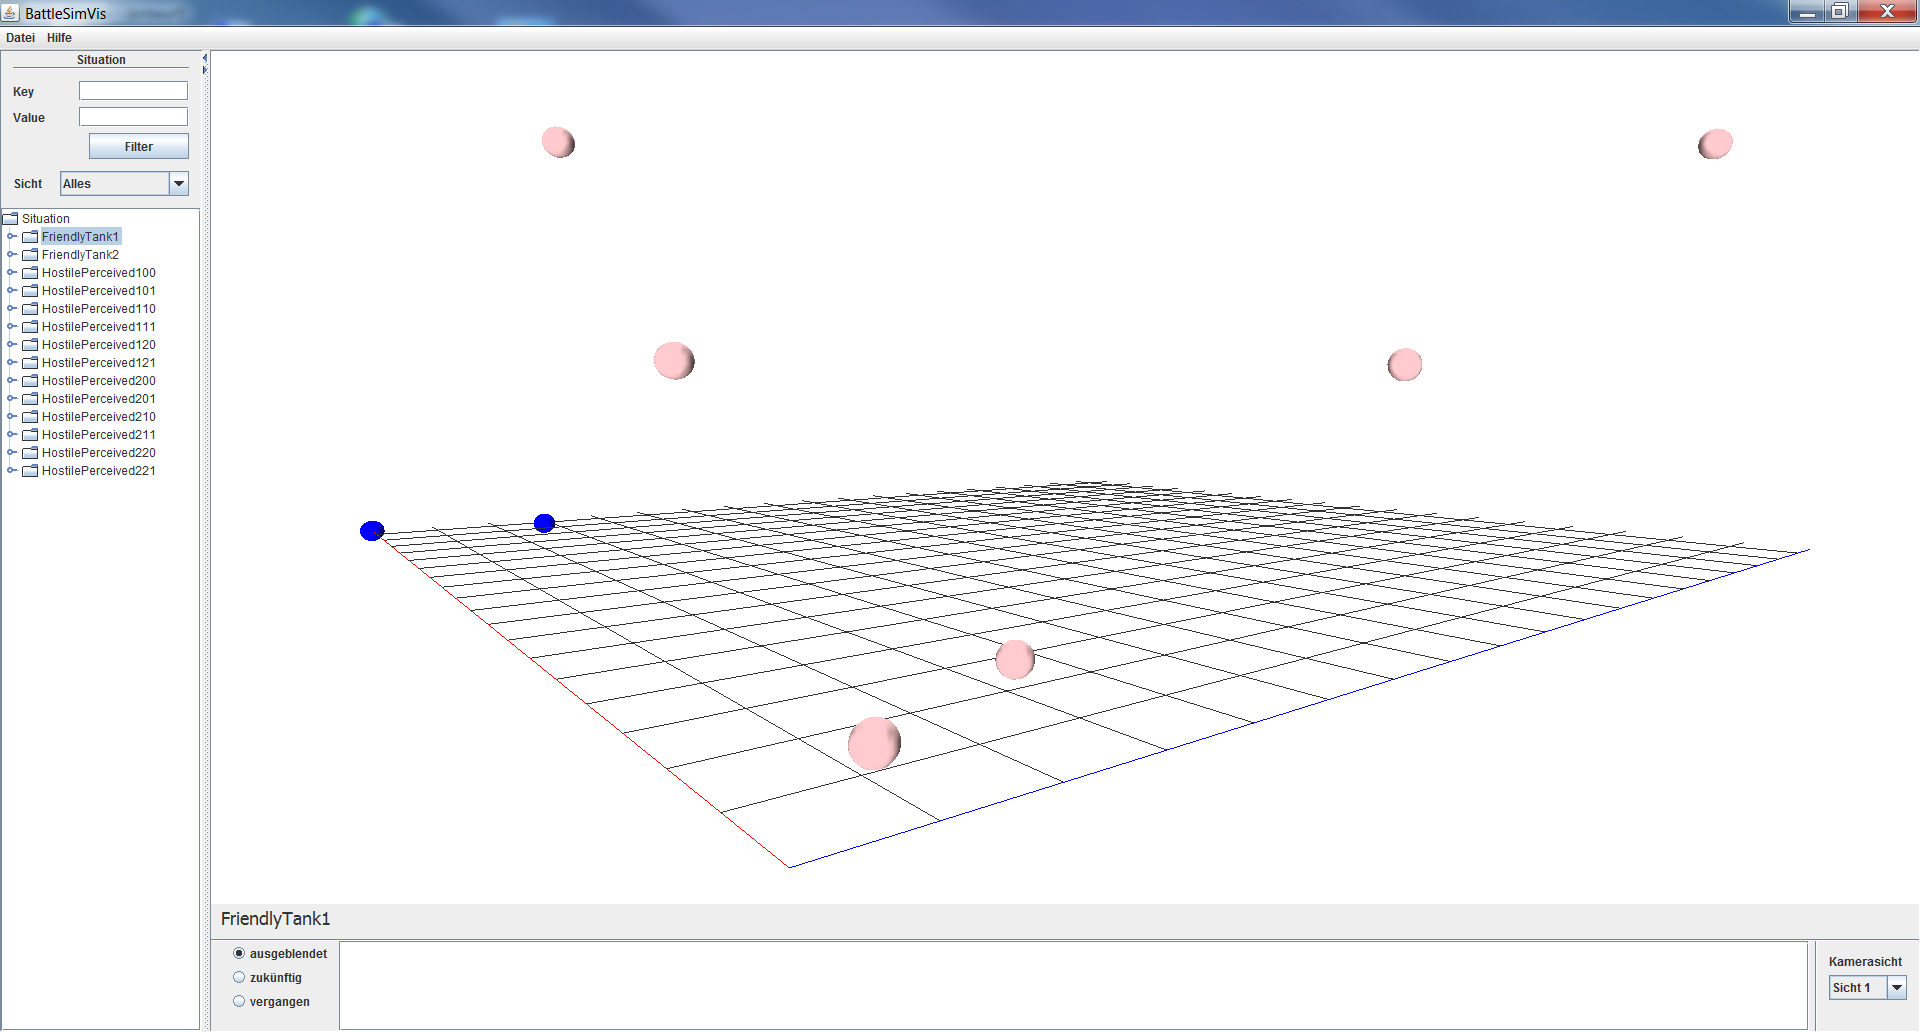
\includegraphics[width=0.90\textwidth]{Bilder/gesamtesFenster.png}
	\caption{BattleSimVis als prototypische Implementierung einer milit�rischen Lagedarstellung}
	\label{fig:gesamtesFenster}
\end{figure}
Dass die oben dargestellten L�sungsans�tze mit Hilfe von Berechnungen umgesetzt werden k�nnen, steht au�er Frage. Mit dem im Folgenden vorgestellten Prototypen soll aber ein anderer Ansatz verfolgt werden: Der S2-Offizier soll mit dem umgesetzten Programm, allein durch die Betrachtung der visualisierten Darstellung, aus den redundanten Daten ein der Realit�t nahe kommendes Lagebild erstellen k�nnen.

\subsubsection{Aufbau der Benutzerschnittstelle}
\label{sec:AufbauDerBenutzerschnittstelle}

Die Benutzeroberfl�che ist in zwei Teile gegliedert. Auf der einen Seite gibt es die textuelle Sicht auf die Lage und alle M�glichkeiten, diese zu manipulieren. Auf der anderen Seite sind die grafische Lagendarstellung in dreidimensionaler Form und die Mittel, diese zu beeinflussen. Welche das im Detail sind, wird im Folgenden beschrieben. Grundlage dieser Aufteilung ist die Struktur, die durch das Visualisierungsframework vorgegeben wird (siehe Abschnitt \ref{ch:Framework}).

\subsubsection{Auswahl der Dimensionen}
\label{sec:AuswahlDerDimensionen}

Um die folgenden �berlegungen und die Grundidee hinter der Visualisierung der Lage im Prototypen zu verstehen, ist es notwendig, zu erkl�ren, welche Dimension im dreidimensionalen Raum mit welcher Gr��e der Daten �bereinstimmt.

Die Ebene, aufgespannt durch L�nge und Breite, spiegelt die Position eines Objekts im Raum wieder. Dabei ist die H�he vernachl�ssigt worden. Da die Eingabedaten in geographischer L�nge und Breite angegeben sind, kommt es hier zu einem, durch die Projektion einer Kugelkappe in die Ebene entstandenen Fehler bez�glich der ma�stabsgetreuen Darstellung von Entfernungen. Wie stark sich dieser auswirkt, wird in Abschnitt \ref{ch:kugelkappe} erl�utert. Dabei ist die Bezeichnung der einzelnen Komponenten eines Vektors an das System von OpenGL angepasst. Das bedeutet, x-Komponente und z-Komponente spannen die Grundebene auf. In Abbildung \ref{fig:gesamtesFenster} ist diese als Gitter gekennzeichnet. Die y-Komponente geht in die H�he. Es handelt sich hierbei um ein rechtsh�ndiges dreidimensionales Koordinatensystem wie in Abbildung \ref{fig:Koordinaten} dargestellt.
\begin{figure}[htb]
	\centering
		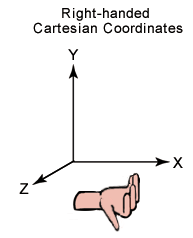
\includegraphics[width=0.35\textwidth]{Bilder/Koordinatensystem.png}
	\caption{Rechtsh\protect\"{a}ndiges Koordinatensystem, wie es OpenGL verwendet \cite{guide}}
	\label{fig:Koordinaten}
\end{figure}

Die dritte Dimension, die man so durch die Vernachl�ssigung der H�he gewinnt, kann durch die Zeit eingenommen werden. Meldungen, die am �ltesten sind, werden direkt auf der durch Gitternetzlinien angezeigten Grundebene dargestellt. Die Anzeige j�ngerer Meldungen erfolgt kontinuierlich inpositive y-Richtung (\emph{in die H�he}).

Der Grund f�r diese Auswahl ist die sp�ter beschriebene M�glichkeit, die Reichweite einer Einheit in Abh�ngigkeit von ihrer H�chstgeschwindigkeit darzustellen.

\subsubsection{Umgesetzte F�higkeiten}
\label{sec:UmgesetzteFaehigkeiten}

\paragraph{Plattformunabh�ngigkeit}
\label{sec:Plattformunabhaengigkeit}
\emph{BattleSimVis} ist plattformunabh�ngig. Es wurde entwickelt um auf allen g�ngigen Betribssystemen zu funktionieren. Getestet ist es mit MS Windows (XP, Vista, 7), MacOS X, Linux (Ubuntu 9.10). Einzige Voraussetzung neben einer aktuellen Java Runtime Environment (mindestens 1.6) ist eine 3D-f�hige Grafikkarte mit zugeh�rigen Treibern. OpenGL in der notwendigen Version ist bereits Bestandteil der genannten Betriebssysteme.

\paragraph{Import der Daten:}
\label{sec:ImportDerDaten}
 \emph{BattleSimVis} ist durch das verwendete Visualisierungsframework in der Lage, Daten im XML-Format zu lesen. F�r den Testgebrauch wurde eine XML-Datenstruktur verwendet, die aus einem Simulationsproxy stammt. Die importierten Daten werden in eine textuelle und eine grafische Ansicht umgewandelt.

\begin{figure}[H]
	\centering
		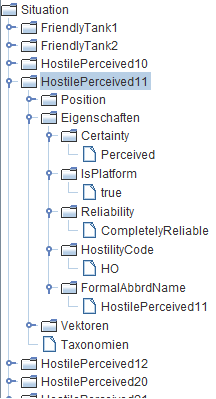
\includegraphics[width=0.20\textwidth]{Bilder/Eigenschaftsansicht.png}
	\caption{Baumstruktur der textuellen Darstellung}
	\label{fig:Eigenschaftsansicht}
\end{figure}


\paragraph{Baumartige Datenanzeige:}
\label{sec:BaumartigeDatenanzeige}
 Die textuelle Anzeige der Daten erfolgt in einer Baumstruktur. Auf erster Ebene befinden sich die Datens�tze, dargestellt durch ihren Bezeichner. Darunter sind f�r jeden Datensatz die eingelesenen Eigenschaften dargestellt.

\paragraph{Dreidimensionale Datenanzeige:}
\label{sec:DreidimensionaleDatenanzeige}
 Im daf�r vorgesehenen Bereich des Prototypen werden die gelesenen Datens�tze im dreidimensionalen Raum dargestellt.

\paragraph{Freie Navigierbarkeit:}
\label{sec:FreieNavigierbarkeit}
 Durch einen Klick in die grafische Visualisierung ist es dem Benutzer m�glich, frei durch den dreidimensionalen Raum zu navigieren. Durch Druck der mittleren Maustaste und Bewegung der Maus kann die Ansicht frei gedreht werden. Die Position des Betrachters wird, �hnlich zu der Steuerung von Computerspielen aus der Ego-Perspektive, mit den Tasten [W], [A], [S] und [D] gesteuert.

\paragraph{Ma�stabsgetreue Abbildung:}
\label{sec:MassstabsgetreueAbbildung}
 Bis auf die oben gemachte Einschr�nkung bez�glich des Fehlers der Projektion einer Kugelkappe in die Ebene, werden die Daten ma�stabsgetreu dargestellt. Die Berechnung der Entfernung erfolgt aufgrund der Tatsache, dass die eigentlichen Koordinaten die Position der Einheit auf einer Kugel beschreiben, durch die in Abschnitt \ref{ch:haversine} dargestellte Haversine-Formel. \\
Die Gitternetzlinien sind auf die importierten Daten angepasst und werden nur in einem notwendigen Bereich auch angezeigt.

\paragraph{Farbige Darstellung der Eigenschaften:}
\label{sec:FarbigeDarstellungDerEigenschaften}
 Um eine milit�rische Lage zu �berblicken, ist die Kenntnis �ber die Zuordnung der Einheiten zu Freund und Feind unabdingbar. Aus diesem Grund stellt \emph{BattleSimVis} feindliche Einheiten in rot und freundliche in blau dar. Weiterhin wird �ber die Helligkeit der Farbe unterschieden, ob es sich um eine echte Einheit (ein meldender eigener Panzer) oder um eine Meldung (einen feindlichen Panzer) handelt. Eine Meldung ist heller, eine echte Einheit wird in einem satten Farbton dargestellt.

\paragraph{Voreingestellte Kameraperspektiven:}
\label{sec:VoreingestellteKameraperspektiven}
 Zus�tzlich zu der freien Navigierbarkeit in der dreidimensionalen Darstellung gibt es die M�glichkeit, zwischen drei vordefinierten Perspektiven auszuw�hlen. Zwei zeigen gegen�berliegende isometrische Ansichten, die dritte stellt die Lage aus einer Draufsicht dar. Dies kann als Ansicht unter Vernachl�ssigung der Zeit-Achse interpretiert werden.

\paragraph{Datenfilter:}
\label{sec:Datenfilter}
 Um die Meldungen auf ein gew�nschtes Ma� zu reduzieren, gibt es die M�glichkeit, die importierten Daten nach bestimmten Eigenschaften auszuw�hlen. Daf�r verf�gt \emph{BattleSimVis}  �ber einen Filter, der anhand von Schl�ssel-Wert-Paaren Datens�tze ausw�hlt. Die Schl�ssel stehen f�r bestimmte Eigenschaften der Meldungen (Freund-Feind-Kennung, Verl�sslichkeit etc.).
 
\begin{figure}[H]
	\centering
		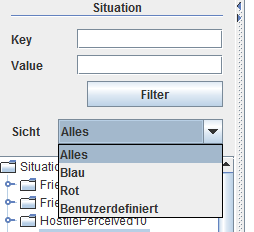
\includegraphics[width=0.30\textwidth]{Bilder/SichtenFilter.png}
	\caption{Filter mit voreingestellten Sichten auf die Lage}
	\label{fig:SichtenFilter}
\end{figure}

\paragraph{Vordefinierte Sichten auf die Lage:}
\label{sec:VordefinierteSichtenAufDieLage}
 Um eine Lage (unabh�ngig von der oben geschilderten Situation des S2-Offiziers) aus der Sicht der roten Einheiten, der blauen Einheiten oder omniscient anzusehen, gibt es vordefinierte Filter. Sie stellen bei der Wahl der blauen Sicht zum Beispiel alle echten blauen Einheiten, aber nur alle gemeldeten roten dar. Im Fall der Feindsicht ist dies genau andersherum. Die omnisciente Sicht zeigt alle Datens�tze.

\paragraph{Selektion in der grafischen Darstellung:}
\label{sec:SelektionInDerGrafischenDarstellung}
 Um die textuelle und die dreidimensionale Sicht optimal miteinander verbinden zu k�nnen, ist es erforderlich, dass eine Auswahl einer Einheit (zum Beispiel zum Inspizieren ihrer Eigenschaften) in beiden Darstellungen vorgenommen werden kann. In der Baumstruktur ist dies trivial durch einen Klick auf den Bezeichner und das damit verbundene Aufklappen des Baums m�glich. \\
Um auch in der grafischen Ansicht die Eigenschaften zu einer Einheit zu erfahren, klickt man sie dort einfach an. Durch einen durchscheinenden gr�nen Kasten wird sie hervorgehoben und in der Baumstruktur wird der dazugeh�rige Pfad expandiert und ausgew�hlt. \\
Dieses F�higkeit wird als Mousepicking bezeichnet und wird in Abschnitt \ref{ch:mousepicking} n�her erl�utert.

\begin{figure}[H]
	\centering
		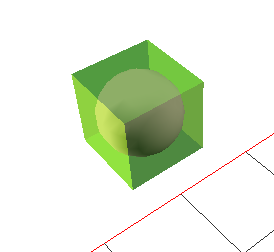
\includegraphics[width=0.20\textwidth]{Bilder/auswahl.png}
	\caption{Hervorhebung in der grafischen Ansicht}
	\label{fig:auswahl}
\end{figure}


\paragraph{Bewegungskegel:}
\label{sec:Bewegungskegel}
 Eine Kernf�higkeit von \emph{BattleSimVis} ist das Einblenden von Bewegungskegeln. Die oben beschriebene Auswahl, welche Eigenschaft einer Meldung auf welche Dimension abgebildet wird, vor allem die Wahl, die Zeit in die H�he zu zeichnen, erm�glicht die Visualisierung der Reichweite einer Einheit. \\
Wird eine Meldung in der grafischen Darstellung ausgew�hlt, kann ein Kegel ein- und ausgeblendet werden, der anzeigt, wo sich eine Einheit in der Zukunft aufhalten kann (nach oben ge�ffneter Kegel) oder in der Vergangenheit aufgehalten haben k�nnte. Alles was innerhalb dieses Kegels liegt, ist in Reichweite der Einheit unter Ber�cksichtigung ihrer Maximalgeschwindigkeit. Alles was au�erhalb ist, kann nicht in der jeweiligen Zeit erreicht worden sein.

\paragraph{Inhalt von Bewegungskegeln:}
\label{sec:InhaltVonBewegungskegeln}
Auch wenn oben beschrieben wurde, dass der S2--Offizier mit Hilfe von \emph{BattleSimVis} allein durch das Ansehen einer Lage Redundanzen ausschalten kann, unterst�tzt das Tool den Anwender bei der Auswertung von Bewegungskegeln, indem es eine Liste aller Einheiten anzeigt, die sich darin befinden.
\begin{figure}[H]
	\centering
		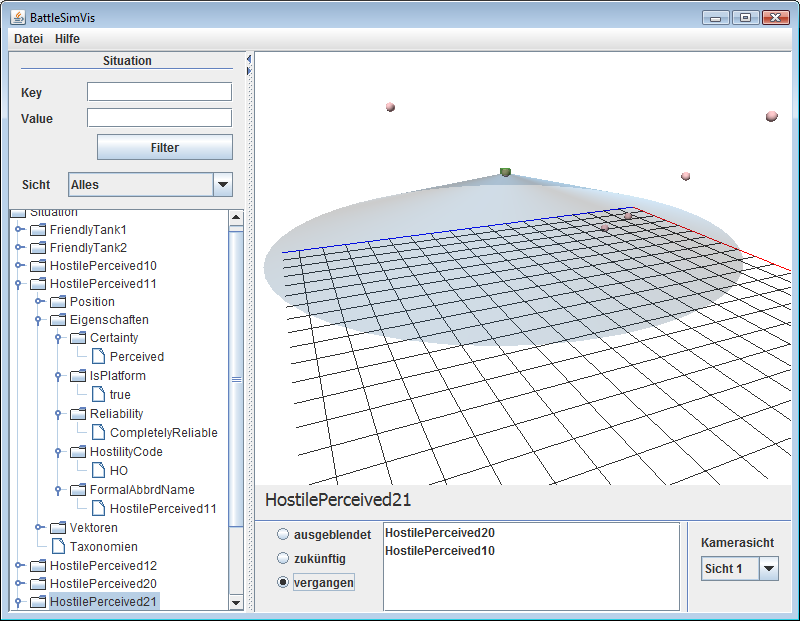
\includegraphics[width=0.50\textwidth]{Bilder/Bewegungkegelverg.png}
	\caption{Bewegungskegel in die Vergangenheit}
	\label{fig:Bewegungkegelverg}
\end{figure}

\subsubsection{Nutzung des Tools zur L�sung des gestellten Problems}
\label{sec:NutzungDesToolsZurLoesungDesGestelltenProblems}
Mit den oben dargestellten F�higkeiten von \emph{BattleSimVis} ist es dem S2-Offizier nun m�glich, die beiden in diesem Abschnitt aufgezeigten L�sungsans�tze zu nutzen, um ein geeignetes Bild von der Lage zu bekommen.

Das Problem der mehrfachen Meldung von Feindeinheiten durch eigene Kr�fte, die gleichzeitig zum Beispiel einen roten Panzer entdecken, wird vom Programm dadurch behoben, dass die Einheiten auch am selben Ort dargestellt werden. Idealerweise sieht der S2-Offizier somit nur einen Panzer, wo auch nur ein Panzer in der Realit�t steht. \\
Weichen die Daten geringf�gig ab, f�llt dies bei Berechnungen auf, jedoch erkennt man Unterschiede in der Position beim Ansehen erst bei so signifikanten Entfernungen, dass es sich um unterschiedliche Einheiten handeln muss.

Um eine Reichweitenanalyse durchzuf�hren, also um zwei zu unterschiedlichen Zeitpunkten gemeldete Objekte eindeutig als auch in der Realit�t nicht identisch zu identifizieren, wird dem S2-Offizier die M�glichkeit an die Hand gegeben, zu jeder Einheit einen in die Zukunft oder einen in die Vergangenheit ragenden Trichter anzeigen zu k�nnen. Damit l�sst sich die theoretische Reichweite eines Objekts anhand der Maximalgeschwindigkeit visualisieren. Alles, was nicht in diesem Trichter ist, muss auch eine andere Einheit sein.

Somit ist gezeigt, dass die prototypische Implementierung durch die gew�hlte Visualisierung die Reduktion redundanter Daten erm�glicht und den S2-Offizier bei der Fusion multisensorischer Daten ad�quat unterst�tzt.

%\section{Erweiterbarkeit und Individualisierbarkeit}


\section{Kernaspekte der Implementierung}
Bei der Umsetzung von Framework und einer prototypischen Implementierung fanden sich einige Implantierungsdetails, die es wert sind, auf sie genauer einzugehen. Dies kann drei Gr�nde haben: Entweder sie sind f�r das Verst�ndnis der Umsetzung relevant (zum Beispiel Abschnitt \ref{ch:mousepicking}), sie beinhalten elegante mathematische Ans�tze (siehe Abschnitt \ref{ch:bewegungskegel}) oder erl�utern andere m�gliche Ans�tze, die aus genannten Gr�nden nicht verfolgt wurden.
\subsection{Observer-Pattern bei abgeleiteten Klassen}
\label{sec:ObserverPatternBeiAbgeleitetenKlassen}
Bei der Auswahl eines Datums in der textuellen Ansicht soll die resultierende Hervorhebung auch in der grafischen Darstellung erfolgen und umgekehrt. Zur Umsetzung dieser Aufgabe empfiehlt sich das Observer-Pattern. 

Dabei gibt es auf der einen Seite eine observierbare Klasse. Dies ist der Ausgangspunkt, an dem die Ver�nderung eines Zustands auftritt. Sie verwaltet eine Liste von Klasseninstanzen, die an dieser Ver�nderung interessiert sind. Geschieht ein Zustands�bergang, werden diese von der observierten Klasse benachrichtigt und k�nnen angemessen reagieren.

Dieses Entwurfsmuster (nach \cite{designpatterns}) ist in Java bereits in die mitgelieferte Klassenbibliothek integriert. Dabei ist der observierte Anteil als Klasse \emph{Observable} fertig umgesetzt. Ein Datenmodell zum Beispiel, das beobachtet werden und in unterschiedlichen Ansichten dargestellt werden soll, wird von der \emph{Observable}-Klasse abgeleitet. Alle notwendigen Methoden werden somit zur Verf�gung gestellt.

Der beobachtende Anteil ist in Java als Interface umgesetzt. Es existiert somit nur ein Ger�st von Methoden. In diesem Fall ist es nur eine einzige, die \emph{update()}-Methode. In ihr muss das Verhalten implementiert werden, das ausgel�st wird, wenn sich an der beobachteten Instanz etwas �ndert.

Dieser von Java bereitgestellte Ansatz kommt an seine Grenzen, wenn die beobachtete Klasse bereits von einer anderen erbt. Denn dann kann sie nicht auch noch von der \emph{Observable} abgeleitet werden. Java verbietet schlie�lich die Mehrfachvererbung von Klassen.

Genau dieses Problem tritt auch bei den beiden Panels ein, die bei der Auswahl von Datens�tzen wechselseitig sowohl Beobachter, als auch Beobachteter sind. Sie sind beide von der Swing-Klasse \emph{JPanel} abgeleitet und d�rfen somit nicht von \emph{Observable} erben.

Zu diesem Problem gibt es zwei unterschiedliche  L�sungsans�tze. Auf der einen Seite kann man ein \emph{Observable}-Interface erstellen, muss dann aber die Liste der Beobachter und die Methoden zum Benachrichtigen selbst implementieren. Dies ist ein nicht unerheblicher Aufwand und zudem unter Umst�nden fehlertr�chtiger Aufwand.

Der andere Ansatz ist, eine innere Klasse in den zu beobachtenden Klassen zu erstellen, die dadurch von \emph{Observable} erben kann und als innere Klasse den vollen Zugriff auf die Instanzvariablen ihrer Umgebung hat. Au�erdem kann die �u�ere Klasse die Methode zum benachrichtigen der Beobachter zum geeigneten Zeitpunkt aufrufen.

So kann mit nur geringen Anpassungen die vorimplementierte L�sung �bernommen und das Problem gel�st werden.

\subsection{Entfernungsberechnung auf der Erde}
\label{ch:haversine}

Der in Abschnitt \ref{ch:Prototyp} vorgestellte Prototyp zur Visualisierung eines Gefechtsfeldes berechnet den Projektionsbereich, indem die minimale und maximale geografische L�nge und Breite der Eingabedaten bestimmt wird. Diese vier Daten beschreiben ein Rechteck, dessen Kantenl�ngen berechnet und in die dreidimensionale Darstellung �bertragen werden.

An dieser Stelle ergibt sich ein Problem aus der Gestalt der Erde in Verbindung mit der Art der Positionsdaten. Weil die Lage der Objekte in Longitude (geografische L�nge) und Latitude (geografische Breite) beschrieben wird, handelt es sich um Koordinaten auf einer Kugel. Daraus ergeben sich Besonderheiten f�r die L�ngenberechnung. 

Weiterhin ist die Erde in Wirklichkeit aber keine Kugel, sondern ein Rotationsellipsoid, der an den Polen einen geringeren Radius hat, als am �quator. Diese Tatsache sei aber f�r die folgenden Betrachtungen zu vernachl�ssigen. Grund daf�r ist die bereits bei der Visualisierung gemachte Vereinfachung, die H�he der Eingabedaten (siehe Abschnitt \ref{ch:kugelkappe}) zu vernachl�ssigen.

Zur Entfernungsberechnung sollen drei Ans�tze aufgezeigt und auf ihre Tauglichkeit untersucht werden. Grundlage hierf�r ist eine Frage aus der U. S. Census Bureau Geographic Information Systems FAQ (\cite{url:USACensus}). Im Hinterkopf sollten dabei folgende Ausma�e bleiben, die vermitteln, in welchen Gr��enordnungen man sich bewegt. Der gr��te Truppen�bungsplatz Europas in Bergen (\cite{wiki:bergen}) hat eine Ausdehnung von 25km x 18km. Er liegt etwa auf 52� n�rdlicher Breite. Ein Kampfpanzer vom Typ Leopard 2A5 hat eine L�nge von 7,72m (\cite{wiki:leopard}).

\subsubsection{Pythagoras}
\label{sec:Pythagoras}
Der erste Ansatz ist die naive Anwendung des Satzes von Pythagoras. Ausgangspunkt  daf�r ist die Annahme, sich nicht auf der Oberfl�che einer Kugel zu bewegen, sondern auf einer Ebene. Dies hat Ungenauigkeiten zur Folge, die in \ref{ch:kugelkappe} beschrieben sind. Der Abstand \emph{d} zweier Punkte berechnet sich somit wie flogt:
\begin{equation}\label{eq:eins}
	d=\sqrt{(x_{2} -x_{1})^2 + (y_{2} -y_{1})^2}
\end{equation}

Der Abstand hat dieselbe Einheit, wie die in kartesischen Koordinaten angegebenen Punkte \emph{P1(x1, y1)} und  \emph{P2(x2, y2)}.

Abh�ngig von der geografischen Breite, an der die Berechnung durchgef�hrt wird, resultieren die in Tabelle \ref{tab:PythagorasFehler} dargelegten Fehler bei einer tats�chlichen L�nge von 20km.

\begin{table*}[ht!]
	\centering
		\begin{tabular}{ | l | l |}
		\hline
			\emph{absoluter Fehler}      & \emph{geografische Breite}       \\ \hline
		  \verb|<| 30m       & \verb|<| 70�        \\ \hline
      \verb|<| 20m      	& \verb|<| 50� \\ \hline
      \verb|<| 9m 				& \verb|<| 30� \\
      \hline
		\end{tabular}
	\caption{Absolute Fehler bei der Entfernungsberechnung nach Pythagoras, Abstand der Punkte ist 20km}
	\label{tab:PythagorasFehler}
\end{table*}

Da die f�r die Veranschaulichung gew�hlte L�nge durchaus in der Realit�t, zum Beispiel auf einem Truppen�bungsplatz auftreten kann, sind die entstehenden Fehler nicht hinnehmbar.

\subsubsection{Seitenkosinussatz}
\label{sec:Seitenkosinussatz}
\begin{figure}[htb]
	\centering
		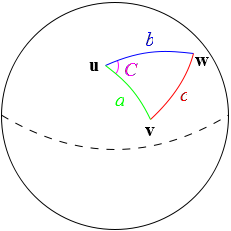
\includegraphics[width=0.30\textwidth]{Bilder/Law-of-haversines.png}
	\caption{Kugeldreieck mit Beschriftung}
	\label{fig:Law-of-haversines}
\end{figure}

Um die Entfernung zweier Punkte auf einer Kugel mathematisch korrekt zu berechnen, behilft man sich der sph�rischen Geometrie. F�r das in Abbildung \ref{fig:Law-of-haversines} dargestellte Kugeldreieck gilt der Seitenkosinussatz:

\begin{equation}\label{eq:zwei}
	\cos{c} = \cos{a} \cos{b} + \sin{a} \sin{b} \cos{C} 
\end{equation}

Dabei soll die Entfernung \emph{c} von Punkt \emph{v} nach Punkt \emph{w} berechnet werden.\\
Nimmt man f�r den Punkt \emph{u} den Nordpol an, und arbeitet auf einer Einheitskugel, dann folgt:

\begin{subequations}\label{grp}
\begin{align}
a&=90^\circ-lat_{1}\label{eq:drei}\\
b&=90^\circ-lat_{2}\label{eq:vier}
\end{align}
\end{subequations}

Bekannt ist folgender Zusammenhang:
\begin{subequations}\label{grp2}
\begin{align}
\sin{90^\circ - x} = \cos{x}\\
\cos{90^\circ - x} = \sin{x}
\end{align}
\end{subequations}

Daraus ergibt sich nach Umformung eine Formel zur Berechnung der L�nge. Das Ergebnis h�ngt von den Einheiten der Eingabedaten ab. Werden die Koordinaten im Gradma� angegeben, so ist zus�tzlich zum Erdradius mit dem Faktor $\frac{\pi}{180^\circ}$ zu multiplizieren. Werden die Daten im Bogenma� eingegeben, entf�llt der letzte Faktor.

Der so berechnete Abstand ist unter Ber�cksichtigung der gemachten Vereinfachung, auf einer Kugel zu rechnen, mathematisch korrekt. Ideal ist diese L�sung jedoch nicht, da die Formel f�r sehr kleine Entfernungen schlecht konditioniert ist. Kritisch ist hier vor allem der Kosinus der L�ngengraddifferenz. Abh�ngig von der Gleitkommapr�zision (weniger als sieben signifikante Stellen) k�nnen bereits L�ngen kleiner einer Bogenminute nicht mehr unterschieden werden. Der Grund hierf�r ist in Tabelle \ref{tab:Kosinus} illustriert.

\begin{table*}[ht!]
	\centering
		\begin{tabular}{ | l | l |}
		\hline
			$x$      & $\cos{x}$       \\ \hline
		  1 Bogenminute       & 0,99999995769202532795126248717334        \\ \hline
      30 Bogensekunden    & 0,99999998942300627605141750356948 \\ \hline
      1 Bogensekunde			& 0,99999999998824778473047407621793 \\
      \hline
		\end{tabular}
	\caption{Schlechte Konditionierung des Kosinus}
	\label{tab:Kosinus}
\end{table*}

\subsubsection{Haversine Formel}
\label{sec:HaversineFormel}

Die gleiche Berechnung wie oben kann durch geeignetes Umstellen der Gleichung auch ohne das geschilderte Problem durchgef�hrt werden. Grundlage bilden die Additionstheoreme und die heute weniger gebr�uchliche trigonometrische Funktion des Semiversus (im englischen Haversine, daher der Name der Formel). 

\begin{equation}
	d = 2 R \arcsin{\sqrt{\sin^2{\frac{lat_{2}-lat_{1}}{2}} + \cos{lat_{1}} \cos{lat_{2}} \sin^2{\frac{\Delta lon}{2}}}}
\end{equation}

Auch diese Formel ist f�r ein spezielles Problem schlecht konditioniert. Problematisch sind Entfernungen zwischen antipodalen Punkten, also Orten, die sich auf dem Erdball gegen�berliegen. Da dieser Fall in Kontext des erstellten Prototyps keine Rolle spielt, ist dieser Fall auch zu vernachl�ssigen. \\
Aus diesem Grund wurde diese Formel zur Entfernungsberechnung verwendet.

\subsection{Informationsverlust durch Projektion einer Kugelkappe auf eine Ebene}
\label{ch:kugelkappe}

Um im vorgestellten Prototyp eine Dimension f�r die Zeit verwenden zu k�nnen, war es notwendig die H�he einer Einheit au�er Acht zu lassen. Dadurch ergibt sich eine Ungenauigkeit, denn die Eingabedaten befinden sich eigentlich auf einer sogenannten Kugelkappe. So bezeichnet man einen Ausschnitt einer Kugeloberfl�che. Durch das Fortlassen der Zeit wird dieser in die Ebene projiziert. 

Um diesen Sachverhalt einfacher durchdenken zu k�nnen, soll er in den zweidimensionalen Raum �bertragen werden. Folglich geht es dann nicht mehr um eine Kugelkappe, die in eine Ebene abgebildet wird, sondern um einen Kreisbogen, der auf eine Gerade projiziert wird.

Durchdenkt man sich diesen Vorgang, ist es klar, dass die resultierende Gerade k�rzer sein muss, als der Kreisbogen. Um diesen Fehler zu veranschaulichen  soll noch einmal die Gr��enordnung des Truppen�bungsplatzes Bergen herangezogen werden. Mit Ausma�en von 25km x 18km ist die theoretisch l�ngste Strecke die Diagonale des aufgespannten Rechtecks. Diese ist nach Pythagoras ca. 30km lang.

Diese 30km als L�nge eines Kreisbogens auf einem Kreis mit einem Radius von 6371km sind der Anhalt f�r die folgende Rechnung. Verbindet man Anfang und Ende des Kreisbogens mit einer Gerade, so ist diese Strecke die gesuchte Projektion.

Zwischen dem Mittelpunkt des Kreises und den Endpunkten des Kreisbogens wird ein gleichschenkliges Dreieck aufgespannt. Das Lot auf der Strecke, dessen L�nge gesucht ist, Teilt das Dreieck in zwei gleichgro�e rechtwinklige Teildreiecke. Grund hierf�r ist, dass das Lot auf der Grundseite eines gleichschenkligen Dreiecks zugleich auch Winkelhalbierende ist. 

Folglich ist der Winkel $\alpha$, der vom Lot und dem Radius, der Mittelpunkt und einen Endpunkt des Kreisbogens verbindet wie folgt zu berechnen:
\begin{subequations}
\begin{align}
\frac{2 \pi \cdot 6371km}{2 \pi} &= \frac{30km}{2 \alpha} \\
\alpha &= \frac{15}{6371}
\end{align}
\end{subequations}
Mit dem berechneten Winkel l�sst sich auf die L�nge der gesuchten Strecke schlie�en. Sie ist das Doppelte der Gegenkathete zum Winkel $\alpha$.
\begin{subequations}
\begin{align}
\sin{\alpha} &= \frac{a}{6371km} \\
l &= 2 \sin{\alpha} \cdot 6371km
\end{align}
\end{subequations}

Die L�nge der Strecke ist somit etwa  29,999972km. Der absolute Fehler betr�gt 2,72cm. Relativ sind das 0,001\,\textperthousand. Das Vernachl�ssigen der H�he f�llt also viel schwerer ins Gewicht, als die beschriebene Vereinfachung.


\subsection{Mousepicking}
\label{ch:mousepicking}
\begin{figure}[hbt!]
	\centering
		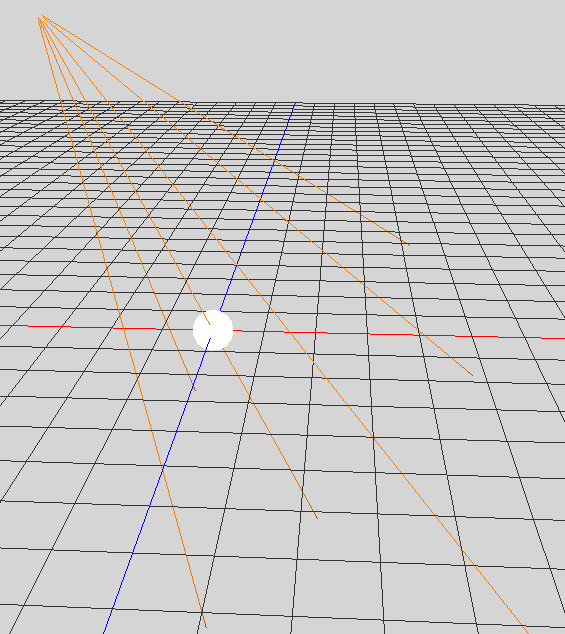
\includegraphics[width=0.30\textwidth]{Bilder/mousepickingscreen.png}
	\caption{Darstellung der von der Maus ausgehenden Strahlen aus \cite{guide}}
	\label{fig:mousepickingscreen}
\end{figure}
Unter dem Wort Mousepicking wird nach \cite{guide} die Auswahl von Objekten in einer dreidimensionalen Darstellung verstanden. Dies ist in der Umsetzung des Visualisierungsframeworks notwendig, wenn ein Datum in der grafischen Ansicht selektiert werden soll, um zum Beispiel seine Eigenschaften in der textuellen Ansicht zu inspizieren.

Bei dieser, auf den ersten Blick sicher trivial erscheinenden T�tigkeit gibt es ein Problem, dass der Leser vielleicht aus der B�ckerei kennt. Zeigt man, vor der Theke stehend, auf ein Geb�ckst�ck hinter der Glasscheibe, welche die Backwaren vor den Kunden sch�tzt, so ist es f�r den/die Verk�ufer/in nicht einfach zu erkennen, auf was gezeigt wird.

Ein �hnlicher Sachverhalt ergibt sich durch das Zeigen mit der Maus auf ein Objekt im dreidimensionalen Raum, denn der Mauszeiger bewegt sich nur auf einer Ebene, einer Art Fenster zum Raum der Darstellung. Um zu berechnen, auf was gezeigt wird, braucht es einen Strahl ausgehend von der Spitze des Mauszeigers. Dasjenige Objekt, das in der k�rzesten Entfernung vom Zeiger getroffen wird, soll ausgew�hlt werden.

Aus der analytischen Geometrie ist aber bekannt [CITE], dass eine Gerade, spezieller aber auch ein Strahl, durch mindestens zwei Punkte zu spezifizieren ist. An dieser Stelle hilft die gew�hlte Grafikengine, indem sie ihrem Benutzer zu einer gew�hlten Bildschirmkoordinate den Startpunkt des Strahls, der von ihr ausgeht, im dreidimensionalen Raum liefert. Zus�tzlich ist sie in der Lage, senkrecht zur Bildschirmebene einen Zielpunkt am Ende des sichtbaren Bereichs zu liefern. Aus diesen beiden Punkten kann nun der f�r das Mousepicking ben�tigte Strahl berechnet werden.

Bei der �bergabe der Bildschirmkoordinaten ist jedoch zu beachten, dass das von Swing verwendete Koordinatensystem seinen Ursprung in der \emph{oberen} linken Ecke besitzt. Im Vergleich zu OpenGL, das den Ursprung mathematisch eing�ngig in der \emph{unteren} linken Ecke platziert. Die y-Koordinate ist also vor der Berechnung von der H�he des Bildschirms abzuziehen. 

In Abbildung \ref{fig:mousepickingscreen} ist eine Visualisierung der Strahlen nachzuvollziehen.

\subsection{Bewegungskegel}
\label{ch:bewegungskegel}
Im der prototypischen Implementierung ist es m�glich, eine Reichweitenanalyse zu einer Einheit durchzuf�hren. Das hei�t, wie weit sie sich unter Annahme einer bestimmten Maximalgeschwindigkeit bewegen kann. Dargestellt wird diese Reichweite durch einen Kegel, der seine Spitze im Ausgangsort der Einheit hat.

Interessant ist es, festzustellen, welche anderen Einheiten sich in dem Kegel befinden. Visuell ist dies meist m�glich, das hei�t eine Berechnung ist nicht immer notwendig. Aber es gibt Grenzf�lle, in welchen eine genaue Aussage nur mathematisch getroffen werden kann. Wie diese Berechnung aussehen kann, soll im Folgenden dargelegt werden. 

\subsubsection{Engine-Mittel}
\label{sec:EngineMittel}

Unter Ber�cksichtigung der Tatsache, dass eine Engine f�r die dreidimensionale Darstellung verwendet wurde, kann man davon ausgehen, dass diese Mittel zur Verf�gung stellt, um das Problem zu l�sen. 

Eine m�gliche Umsetzung basiert auf der Technik, die auch f�r die Mousepicks (siehe Abschnitt \ref{ch:mousepicking}) verwendet wurde: Gegeben seien die dreidimensionalen Objekte der Einheiten und der Kegel, in dem sie potentiell liegen k�nnten. Von jeder Einheit wird jetzt ein Strahl ausgesendet. Richtung ist grunds�tzlich die negative y-Richtung. Naiv gesprochen: \emph{nach unten}. 

Genau wie beim Mousepicking wird jetzt gepr�ft, ob der Kegel getroffen wurde. War dies der Fall, befindet sich die Einheit darin. 

In der prototypischen Implementierung wurde diese Variante nicht umgesetzt. Grund daf�r ist sind Probleme mit dem Algorithmus, den die Engine f�r die Kollisionsberechnung nutzt. Er ist auf Geschwindigkeit, nicht jedoch auf Genauigkeit ausgelegt. Ziel der Berechnung sollte aber ein sehr genaues Ergebnis sein. Deswegen entf�llt diese Variante.

\subsubsection{Winkelvergleich}
\label{sec:Winkelvergleich}

Ein Ansatz das Problem mit Analytischer Geometrie anzugehen, ist der Vergleich von Winkeln zwischen Vektoren. F�r diese Variante kann o. B. d. A. der Kegel als (gleichschenkliges) Dreieck angenommen werden. Auf der Basis wird nun das Lot gef�llt. Bei diesem handelt es sich um die H�he des Dreiecks. 

Als Erstes wird der Winkel zwischen den Schenkeln des Dreiecks und dem Lot berechnet. Da der Radius des Kegels mit der H�he des Dreiecks (und ebenfalls der H�he des Kegels) ein rechtwinkliges Dreieck aufspannt, gilt:
\begin{subequations}\label{eq:tan}
\begin{align}
\tan{\alpha} &= \frac{r}{h} \\
\alpha &= \arctan{\frac{r}{h}}
\end{align}
\end{subequations}

Als Zweites wird der Winkel berechnet, der sich f�r jede zu pr�fende Einheit zwischen der Strecke von der Spitze des Kegels zur Einheit und dem Lot befindet. Er berechnet sich nach:
\begin{equation}\label{eq:winkel}
\cos{\beta} = \frac{\vec{a}\bullet\vec{b}}{\left|\vec{a}\right| \cdot \left|\vec{b}\right|} \\
\end{equation}

Ist dieser Winkel gr��er, liegt die Einheit au�erhalb des Kegels. Ist er anderenfalls kleiner, befindet sich die gepr�fte Einheit im Kegel. 

Insgesamt handelt es sich hierbei um ein recht rechenaufwendiges Verfahren, da es f�r jede Einheit durchgef�hrt werden muss. Aus diesem Grund stellt sich die Frage, ob das es M�glichkeiten zur Vereinfachung gibt.

Vergleich der y-Komponenten
Berechnet man den Winkel $\alpha$ nicht mit der Gleichung \ref{eq:tan}, sondern mit Gleichung \ref{eq:winkel}, ergibt sich eine Vereinfachung: Da der Richtungsvektor nur in der y-Komponente von null verschieden ist, geht auch nur die y-Komponente des Schenkelvektors ein. Damit degeneriert das Skalarprodukt zu einer einzigen Multiplikation. 

F�r die Winkelbrechnung sind die L�ngen der Vektoren, die f�r die Berechnung herangezogen werden, unerheblich. Darum muss f�r das Lot nicht mit dem Vektor (0, h, 0) gerechnet werden. Es gen�gt (0, 1, 0). Das Skalarprodukt muss nun schlicht nicht mehr ausgerechnet werden.

Ebenso k�nnen der Schenkelvektor und der Vektor von der zu pr�fenden Einheit Richtung Kegelspitze normalisiert werden. Resultat ist, dass der Nenner der Formel zur Winkelberechnung gleich eins ist. Die Berechnung des Arkuskosinus ist zum Vergleich der beiden Winkel hinf�llig. Schlie�lich m�sste er nur von den y-Komponenten berechnet werden. Diese k�nnen aber auch gleich verglichen werden: Ist die des normalisierten Vektors der zu pr�fenden Einheit kleiner, liegt sie au�erhalb. Ist die des normalisierten Schenkelvektors kleiner, liegt sie im Kegel.

Zusammenfassen m�ssen zur Berechnung nur noch folgende Schritte durchlaufen werden: 
\begin{enumerate}
	\item Einmalige Berechnung des Schenkelvektors
	\item Normalisierung des Schenkelvektors
	\item F�r jede zu pr�fende Einheit:
\begin{enumerate}
	\item Berechnung des Vektors von ihr zur Kegelspitze
	\item Normalisierung dieses Vektors
	\item Vergleich der y-Komponenten der beiden Vektoren.
\end{enumerate}
\end{enumerate}

Durch diese Optimierung werden pro zu pr�fender Einheit folgende absoluten und relativen Einsparungen gemacht:
\begin{table*}[ht!]
	\centering
		\begin{tabular}{ | l | l |}
		\hline
			\emph{absolute Verbesserung}      & \emph{relative Verbesserung} 	      \\ \hline
		  -4 Additionen       							& -44\%        												\\ \hline
      -6 Multiplikationen    						& -66\% 															\\ \hline
      -3 Divisionen											& -50\% 															\\ \hline
      -1 Wurzel    											& -50\% 															\\ \hline
      -1 trigonometrische Funktion    	& -100\% 															\\ \hline
		\end{tabular}
	\caption{Erreichte Verbesserungen durch Vereinfachung der Berechnung}
	\label{tab:verbesserungen}
\end{table*}




%----------------------------------------------------------------%
% fazit.tex						    		  	    										       %
%----------------------------------------------------------------%
\chapter{Fazit und Ausblick}
In diesem letzten Kapitel soll eine Bewertung der im Rahmen dieser Arbeit entstandenen Implementierung vorgenommen werden. Dazu werden die zu Beginn gesetzten Ziele als Ma�stab genommen. Anschlie�end soll aufgezeigt werden, welche Aspekte in einer weiterf�hrenden Arbeit aufzugreifen sind und wie das Erstellte eingesetzt werden kann. 

\section{Bewertung}
Ziel dieser Arbeit sollte ein plattformunabh�ngiges Framework sein, das die Visualisierung von multisensorischen Daten erm�glicht. Es sollte einer prototypischen Implementierung dienen, welche Daten eines Gefechtssimulators darstellen kann und die Redundanzen in ihnen durch Visualisierung zu beseitigen vermag.

Das Ergebnis der Arbeit ist vielversprechend. Im Prinzip konnten alle Ziele umgesetzt werden. Inwieweit dies geschehen ist, wird im Folgenden f�r die einzelnen Aspekte dargelegt.

\subsubsection{Framework zur Visualisierung von Multisensorischen Daten}
\label{sec:FrameworkZurVisualisierungVonMultisensorischenDaten}

Im Zuge der Implementierung  ist ein Klassenger�st entstanden, das aus drei Teilen besteht. Der erste ist eine Datenstruktur, die durch ihre modulare Struktur eine hohe Flexibilit�t und Erweiterbarkeit bietet. Weiterhin ein Backend, welches auf der einen Seite den einfachen Import von \gls{xml}-Dateien in die geschaffene Datenstruktur erm�glicht und auf der anderen Seite diese mit weitreichenden M�glichkeiten der Individualisierung in eine dreidimensionale Ansicht umformen kann. Im dritten Teil, dem Frontend, k�nnen die Daten visuell und textuell betrachtet werden. Es ist also ein funktionsf�higes Framework entstanden.

\subsubsection{Prototypische Implementierung}
\label{sec:PrototypischeImplementierung}

Mit Hilfe des erstellten Klassenger�sts war es ohne hohen Implementierungsaufwand m�glich, die vom Betreuer dieser Arbeit zur Verf�gung gestellten Daten eines Gefechtssimulatorproxy darzustellen. Entstanden ist dabei ein Prototyp, der in der Lage ist, Datens�tze mit ihren Eigenschaften anzuzeigen.

\subsubsection{Beseitigung von Redundanzen durch Visualisierung}
\label{sec:BeseitigungVonRedundanzenDurchVisualisierung}

Fusion auf Basis von Datens�tzen, die sich an einer Stelle befindlichen, geschieht im Prototyp automatisch, da sie visuell nicht unterscheidbar sind und somit als ein Datum zu erkennen sind.

Weiterhin wurde durch die Darstellung von Bewegungskegeln eine M�glichkeit der Reichweitenanalyse geschaffen. Somit ist es m�glich, auch Sichtungen, die zu unterschiedlichen Zeiten an unterschiedlichen Orten gemacht wurden, einem Objekt zuzuordnen. Zusammenfassend ist somit mit dem Prototyp ein m�chtiges Werkzeug zur Visualisierung und visuellen Fusion von Daten entstanden.

\subsubsection{Plattformunabh�ngigkeit}
\label{sec:fazitPlattformunabhaengigkeit}

Aufgrund der Umsetzung in Java, der Verwendung von Swing und einer Grafikklassenbibliothek, die f�r alle g�ngigen Betriebssysteme vorhanden ist, entstand ein plattformunabh�ngiges System. Der Prototyp wurde erfolgreich auf Microsoft-Systemen (Windows XP, Vista, 7), auf Linux-Systemen (Ubuntu 9.04/9.10) und MacOS X getestet. Beschr�nkt wird die Unabh�ngigkeit nur von der Verf�gbarkeit nativer \gls{lwjgl}-Bibliotheken und der \gls{opengl}-F�higkeit des Betriebssystems. Da letztere f�r Windowssysteme bereits ab Win98 der Fall ist, scheitert es daran sicher mit sehr geringer Wahrscheinlichkeit.

\section{Weiterf�hrende Arbeit}
Obwohl die Ziele der Arbeit sind erf�llt worden sind, gibt es dennoch Ans�tze f�r die weiterf�hrende Arbeit und Punkte, die sicher noch verbessert werden k�nnen. Diese beiden Aspekte sollen im Folgenden beleuchtet werden.

\subsubsection{Ans�tze zur Verbesserung}
\label{sec:AnsaetzeZurVerbesserung}

Das gr��te Problem dieser Arbeit war die kurze Zeit, in der sie erstellt werden musste. Aus diesem Grund mussten an einigen Stellen Abstriche gemacht werden. Als besonders kritisch ist dabei das Vertrautmachen mit der verwendeten Grafikbibliothek (siehe Abschnitt \ref{sec:jme}). Zwar hat sie sich in ersten Experimenten als sehr leicht verst�ndlich und einfach zu handhaben gezeigt. Das an einigen Stellen jedoch ben�tigte Wissen von der vollen Komplexit�t hat aber gefehlt.

Konkret �u�ert sich dieses Problem in den zwei separaten Datenmodellen. Auf der einen Seite steht das mit dem Framework entwickelte eigene Datenmodell. Auf der anderen Seite gibt es den Szenenbaum zum Anzeigen der Daten. Werden Informationen zu einem grafischen Objekt ben�tigt, muss im Datenmodell des Frameworks ein Lookup geschehen. Dieser Vorgang ist aufwendig und kann beseitigt werden, indem beide Datenmodelle verschmelzen. Dabei m�ssen lediglich die Klassen zur Datenspeicherung von den Knoten des Szenenbaums erben. Derart tiefgreifende Struktur�nderungen sollten aber zum Ende der Arbeit nicht mehr durchgef�hrt werden. Die ungewollten Nebenwirkungen waren nicht absch�tzbar.

Ebenfalls durch die kurze Zeit, die f�r diese Arbeit zur Verf�gung stand, entwickelten sich redundante Strukturen innerhalb des Klassenger�sts. Zum Wohle eines funktionsf�higen Prototyps wurde an einigen Stellen die Eleganz des Entwurfs in den Hintergrund ger�ckt. Durch den geeigneten Einsatz von Refactoring ist dieser Missstand jedoch zu beseitigen.

Ein weiterer Punkt, an dem Verbesserungen vorgenommen werden k�nnen, ist die Ergonomie des Prototyps. Das auff�lligste Beispiel ist die in Abschnitt \ref{sec:Datenfilter} beschriebene Filterfunktion. Der Name des Schl�ssels, nach dem gefiltert werden soll, muss in korrekter Gro�- und Kleinschreibung von Hand eingegeben werden. F�rderlich w�re hier, eine Liste mit den m�glichen Eigenschaften bereits aus den Daten auszulesen und mit Hilfe dieser Liste eine Auswahl zu erm�glichen.

\subsubsection{Weiterf�hrende Ans�tze}
\label{sec:WeiterfuehrendeAnssaetze}


Der n�chste Schritt muss, vor allem im Hinblick auf die Erprobung des Frameworks, die Visualisierung eines anderen Datenbestandes sein. Einige M�glichkeiten sollen hier aufgez�hlt werden:

\paragraph{Neighbor Discovery Protocol}
\label{sec:NeighborDiscoveryProtokoll}

\gls{ndp} ist ein Protokoll, das unter anderem die �bersetzung von \gls{ip}v6-Adressen in Link-Layer-Adressen leistet. Es entspricht zum Address Resolution Protocol in \gls{ip}v4-Netzen.

\cite{thomas1} und \cite{thomas2} entwickeln einen Monitoring-Ansatz f�r \gls{ndp}. In diesem Zusammenhang entstand die Idee, die anfallenden Daten zu visualisieren. Als Dimensionen k�nnten jeweils die \gls{ip}v6- und \gls{mac}-Adressen, sowie die Zeit,  dienen. Daraus k�nnten Schl�sse �ber h�ufig verwendete Hersteller der Netzhardware gezogen werden. Auch k�nnten Informationen gewonnen werden, welche Benutzer des Netzwerks aufgrund von h�ufigem Adresswechsel im Netz verd�chtig erscheinen. 

\paragraph{Internethandel}
\label{sec:Internethandel}

Eine weitere M�glichkeit, die Visualisierung von Daten zu nutzen, ist das Auswerten vom Kaufverhalten bei Kunden von Online-Shops und das Surf-Verhalten von Internet-Nutzern. Theoretisch l�sst sich bei geeigneter Visualisierung ein Verhaltensmuster erkennen. Dieses k�nnte dazu dienen, Kunden auf unterschiedlichen Plattformen wiederzuerkennen. Hier w�re die Visualisierung wieder zur Datenfusion eingesetzt. 

\subsubsection{Milit�rische Lagen}
\label{sec:MilittaeischeLagen}

Auf diesem Gebiet bewegt sich zwar schon der Prototyp, aber es gibt eine Vielzahl von M�glichkeiten, hier weiterf�hrende Arbeit zu bestreiten. Ein Ansatz ist das Verbessern der Reichweitenanalyse. Fahrzeuge k�nnen nicht auf jedem Untergrund ihre Maximalgeschwindigkeit erreichen. Darum k�nnten Informationen �ber die Gel�ndebeschaffenheit in die Visualisierung mit einflie�en. Das h�tte zur Folge, dass nicht mehr echte Trichter gezeichnet werden. Sie w�rden an einigen  Stellen, in Abh�ngigkeit vom Terrain, deformiert. Die Berechnung solcher Gebilde wird den anspruchvollsten Teil der Arbeit ausmachen.

Zus�tzlich k�nnte der Prototyp, neben der vorhandenen visuellen Fusion, um mathematische Modelle erweitert werden. Einen gro�en Einfluss werden dabei statistische und stochastische Berechnungen haben, da die Daten immer mit einer gewissen Unsicherheit behaftet sind. 


\section{Fazit}
Zusammenfassend ist in dieser Arbeit ein Prototyp zur Visualisierung einer milit�rischen Lage entstanden, der die in ihn gesetzten Anforderungen erf�llt. Durch Abstraktion des Prototyps konnte ein Klassenger�st erstellt werden, das f�r die Implementierung weiterer Datenarten verwendet werden kann.

Die erhoffte F�higkeit, Redundanzen in multisensorischen Daten durch Visualisierung beseitigen zu k�nnen, wurde umgesetzt. Bei der Erprobung mit echten, sowie konstruierten Eingabedaten hat sie sich als m�gliche Alternative zu den grundlegenden mathematischen Modellen herausgestellt. Welche  Qualit�t der verfolgte Ansatz hat, bleibt in weiterf�hrender Arbeit unter Beweis zu stellen.


\singlespacing

\cleardoublepage
\phantomsection
\addcontentsline{toc}{chapter}{Literaturverzeichnis}
\bibliographystyle{geralpha}
\bibliography{literatur}

\cleardoublepage
\printglossary[type=\acronymtype,toctitle=Abk�rzungsverzeichnis,title=Abk�rzungsverzeichnis,style=long]

\cleardoublepage
\phantomsection
\addcontentsline{toc}{chapter}{Abbildungsverzeichnis}
\listoffigures

\cleardoublepage
\phantomsection
\addcontentsline{toc}{chapter}{Tabellenverzeichnis}
\listoftables

\cleardoublepage
\phantomsection
\addcontentsline{toc}{chapter}{Listingverzeichnis}
\lstlistoflistings
\cleardoublepage
\phantomsection

\appendix

\addcontentsline{toc}{chapter}{Anhang}
\chapter{Inhalt der CD}
Die beigelegte CD enth�lt alle Programme, die zum Ausf�hren der Testanwendungen ben�tigt werden. Es ist nat�rlich auch m�glich,
aktuellere Versionen der Software aus dem Internet herunterzuladen. Eine Installationsanleitung f�r die zum Einsatz kommenden
Programme folgt in Anhang B.

\subsubsection{Inhalt:}

\begin{center}
\begin{longtable}{|l|l|l|} \hline
	Datei 												& Format 	& Bemerkungen 														\\ \hline
	Diplomarbeit									& pdf			& Eine digitale Kopie der Diplomarbeit 		\\ \hline
	Zwischenpr�sentation					&	pdf			& PDF Version der Zwischenpr�sentation 		\\ \hline
	Endpr�sentation								& pdf			& PDF Version der Endpr�sentation					\\ \hline
	Java JDK 6										& exe			& Offline-Installation des JDK 6 Update 16 \\ \hline
	Java JRE 6										& exe			& Offline-Installation des JRE 6 Update 16 \\ \hline
	Eclipse Galileo								& zip			& Eclipse 3.5 mit RCP											\\ \hline
	PluginCore										& jar			& MgmtPlugin-Kern Version 1.0.0						\\ \hline
	de.inf06.dcl									& Project	&	Java Source des DCL											\\ \hline
	de.inf06.plugin.core					& Project & Java Source des MgmtPlugin-Kerns				\\ \hline
	de.inf06.plugin.demo					& Project & Java Source eines Beispielplugins				\\ \hline
	de.inf06.plugin.guiprovider		& Project & Java Source des GUIProvider-Plugins			\\ \hline
	de.inf06.plugin.mappingeditor & Project & Java Source eines Beispielplugins				\\ \hline
	de.inf06.plugin.snmp					& Project & Java Source eines Beispielplugins				\\ \hline
	ManagementFramework						& Project & Java Source des MgmtFrameworks					\\ \hline
	org.jacorb.essentials					& Project & RCP Plug-in f�r GUIProvider							\\ \hline
	org.openorb.trader						& Project	& RCP Plug-in f�r GUIProvider							\\ \hline	
	JacORB Source									& zip			& JacORB Version 2.3.1 Full Source				\\ \hline
	JacORB Binaries								& zip			& JacORB Version 2.3.1 Binaries						\\ \hline
	OpenORB ORB Source						& zip			& OpenORB ORB Version 1.4.0 Full Source		\\ \hline
	OpenORB ORB Binaries					& zip			&	OpenORB ORB Version 1.4.0 Binaries			\\ \hline
	OpenORB Services							& zip			& ConcurrencyControlService								\\
																&					& EvaluatorUtility												\\
																&					& EventService														\\
																&					&	InterfaceRepository											\\
																&					& ManagementBoard													\\
																&					& NamingService														\\
																&					& NotificationService											\\
																&					&	PersistentStateService									\\
																&					& PropertyService													\\
																&					& SSL																			\\
																&					&	TimeService															\\
																&					& Tools																		\\
																&					& TradingService													\\
																&					& TransactionService											\\
																&					& Full Source und Binaries								\\ \hline
	Apache LOG4J									& jar			& LOG4J Version 1.2.15										\\ \hline
	SNMP4j												& jar			& SNMP4J Version 1.10.1										\\ \hline	
\end{longtable}
\end{center}

\cleardoublepage

%\chapter{Installationsanleitungen}
An dieser Stelle wird erl�utert, wie die mitgelieferte Software zu installieren und zu konfigurieren ist. Erfahrene Benutzer
k�nnen diesen Teil �berspringen und die Software nach ihren Vorlieben installieren. Dieser Teil dient nur als Anhalt und hat
nicht den Anspruch einer vollst�ndigen Anleitung. Vielmehr werden die wichtigsten Schritte erl�utert und eine M�glichkeit zur
Konfiguration aufgezeigt.

Die entsprechenden Programme auf der beiliegenden CD sind f�r ein Windowsbetriebssystem ausgelegt. Das Testsystem war dabei
Windows XP SP 2 32-bit. Die Software ist auch unter anderen Betriebssystemen erh�ltlich. F�r eine Installationsanleitung f�r weitere
Betriebsysteme wird auf das Internet verwiesen.

\section{Java}

\begin{enumerate}
	\item F�hren Sie die Datei \emph{jdk-6u16-windows-i586.exe} aus.
	\item Sollte sich eine Sicherheitswarnung �ffnen, w�hlen Sie "`Ausf�hren"'.
	\item Folgen Sie den Anweisungen des Installationsdialogs.
	\item F�gen Sie nach der Installation die Umgebungsvariable \emph{JAVA\_HOME} hinzu, falls diese noch nicht existiert: \\
		Start $\Longrightarrow$ Systemeinstellungen $\Longrightarrow$ System $\Longrightarrow$ Erweitert $\Longrightarrow$ Umgebungsvariablen 
		$\Longrightarrow$ Systemvariablen $\Longrightarrow$ Neu \\
		Der Inhalt der Variable ist das Installationsverzeichnis des JDK. Nach der Ver�nderung muss die Konsole neu gestartet werden.
	\item F�gen Sie das Verzeichnis "`\$JAVA\_HOME\$/bin"' der PATH Variable hinzu.
	\item Falls gew�nscht, kann nun noch die Datei \emph{jre-6u16-windows-i586.exe} ausgef�hrt werden.
	\item Der Installationsverlauf ist analog, jedoch ist keine weitere Variable n�tig.
	\item Starten Sie Ihr System neu.
\end{enumerate}

\section{Eclipse}

\begin{enumerate}
	\item Entpacken Sie die Datei \emph{eclipse-rcp-galileo-win32.zip} mit einem Programm Ihrer Wahl in ein Verzeichnis Ihrer Wahl.
	\item F�hren Sie die \emph{eclipse.exe} im Verzeichnis "`eclipse"' aus.
	\item Definieren Sie einen Ordner als Ihren Workspace.
	\item Installieren Sie das EclipseCORBA Plug-in: \\
		Help $\Longrightarrow$ Install New Software ... $\Longrightarrow$ Add \\
		Name: EclipseCORBA \\ 
		Location: http://eclipsecorba.sf.net/update \\
		W�hlen Sie alle Items im Men� aus und folgen Sie dem Dialogverlauf.
\end{enumerate}

\section{JacORB}

\begin{enumerate}
	\item Entpacken Sie die Datei \emph{jacorb-2.3.1-src.zip} mit einem Programm Ihrer Wahl in ein Verzeichnis Ihrer Wahl.
	\item F�gen Sie die Variable \emph{JACORB\_HOME} zu den Umgebungsvariablen des Systems hinzu.
	\item F�gen Sie das Verzeichnis "`\$JACORB\_HOME\$/bin"' der PATH Variable hinzu.
	\item �ffnen Sie die Datei \emph{orb.properties} im Verzeichnis "`\$JACORB\_HOME\$/etc"' mit einem Programm Ihrer Wahl.
	\item �ndern Sie die Variable \emph{jacorb.config.dir} auf "`\$JACORB\_HOME\$/etc"' ab.
	\item �ndern Sie die Variable \emph{ORBinitRef.NameService} ab, auf einen Ordner Ihrer Wahl mit Schreibrechten. Es ist m�glich
		die Voreinstellung mit "`file:/c:/NS\_Ref"' beizubehalten.
	\item �ndern Sie die Variable \emph{jacorb.naming.ior\_filename} ab, auf den selben Ordner wie \emph{ORBinitRef.NameService}.
	\item Kopieren Sie die ge�nderte \emph{orb.properties} in Ihr Benutzerverzeichnis, in "`\$JAVA\_HOME\$/lib"' und in "`\$JAVA\_HOME\$/jre6/lib"'
	\item Ersetzen Sie beim Kopiervorgang eine eventuell bereits vorhandene \emph{orb.properties}.
	\item �ffnen Sie die Datei \emph{jacorb.properties} im Verzeichnis "`\$JACORB\_HOME\$/etc"' mit einem Programm Ihrer Wahl.
	\item �ndern Sie analog die Variable \emph{jacorb.naming.ior\_filename} und die Variable \emph{ORBinitRef.NameService}.
	\item Testen Sie die Einstellungen, indem Sie die Konsole aufrufen. Bei Eingabe des Kommandos ns, sollte der NameServer von JacORB starten.	
	\item Bei weitergehender Konfiguration konsultieren Sie die Datei ProgrammingGuide.pdf im Verzeichnis "`\$JACORB\_HOME\$/doc"'
\end{enumerate}

\section{OpenORB}

\begin{enumerate}
	\item Kopieren Sie aus dem Verzeichnis "`CD:/OpenORB"' alle Ordner bis auf den Ordner \emph{src} in ein Verzeichnis Ihrer Wahl.
	\item F�gen Sie die Variable \emph{TCOO\_HOME} zu den Umgebungsvariablen des Systems hinzu. Diese enth�lt das Verzeichnis, in das Sie
		die Ordner kopiert haben.
	\item �ffnen Sie im Verzeichnis "`\$TCOO\_HOME\$/OpenORB/config"' die Datei \emph{OpenORB.xml} mit einem Programm Ihrer Wahl.
	\item Editieren Sie die Datei, wie im unten stehenden Listing zu erkennen. 
	\item Geben Sie folgende Kommandos in die Konsole ein: \\
		cd \$TCOO\_HOME\$/tools/bin \\
		updateConfig OpenORB OpenORB.xml
	\item �ffnen Sie im Verzeichnis "`\$TCOO\_HOME\$/OpenORB/config"' die Datei \emph{trader.xml} mit einem Programm Ihrer Wahl.
	\item �ndern Sie den Namen des TradingServers in einen beliebig gew�hlten Namen um.
	\item Geben Sie folgende Kommandos in die Konsole ein: \\
		cd \$TCOO\_HOME\$/tools/bin \\
		updateConfig TradingService trader.xml
	\item Erstellen Sie eine Batchdatei mit folgendem Inhalt: \\
		cd \$TCOO\_HOME\$
		java \\
		-Xbootclasspath/p:/OpenORB/lib/endorsed/openorb\_orb\_omg-1.4.0.jar \\
		-Dopenorb.home.path=\$TCOO\_HOME\$ \\
		-jar /tools/lib/launcher.jar org.openorb.trader.Server
	\item Ab dem Kommando \emph{java} muss alles in einer Zeile stehen.
	\item Der Aufruf dieser Datei startet den Trading Server, der auf den JacORB Naming Server zugreift.
\end{enumerate}

\begin{verbatim}
...
<profile name="default" xlink:href="$(openorb.home)config/
default.xml#default">
  <property name="NameService" value="file:/c:/NS_Ref" />
</profile>
...
\end{verbatim}

\section{Managementframework}

\begin{enumerate}
	\item �ffnen Sie Eclipse.
	\item Importieren Sie das Projekt \emph{ManagementFramework} in Ihren Workspace: \\
		File $\Longrightarrow$ Import $\Longrightarrow$ Existing Projects into Workspace \\
		W�hlen Sie das Verzeichnis "`CD:/Implementierung/ManagementFramework"' als \emph{root directory}. \\
		Best�tigen Sie dies mit \emph{Finish}.
	\item Passen Sie im \emph{Build Path} des Projekts die Referenz auf die log4j-1.2.15.jar entsprechend ihres Systems an.
	\item �ffnen Sie das \emph{Run} Profil der Klasse \emph{start/starter.java}: \\
		Rechtsklick auf starter.java $\Longrightarrow$ Run As $\Longrightarrow$ Run Configurations... 
	\item Geben Sie im Tab \emph{Arguments} im Feld \emph{VM arguments} Folgendes ein: \\
		-Djava.endorsed.dirs=[PATH\_TO\_JACORB]/bin \\
		-Djacorb.home=[PATH\_TO\_JACORB]
	\item F�gen Sie im Tab \emph{Classpath} unter \emph{Bootstrap Entries} folgende externe JARs hinzu: \\
		backport-util-concurrent.jar \\
		jacorb.jar \\
		logkit-1.2.jar \\
		slf4j-api-1.5.6.jar \\
		slf4j-jdk14-1.5.6.jar \\
		Diese befinden sich im Verzeichnis "`\$JACORB\_HOME\$/lib"'.
	\item Best�tigen Sie mit \emph{Apply} und f�hren Sie die starter.java mit \emph{Run} aus.
\end{enumerate}

\section{PluginCore Source}
	
\begin{enumerate}
	\item �ffnen Sie Eclipse.
	\item Importieren Sie das Projekt \emph{de.inf06.plugin.core} in Ihren Workspace. 
	\item Passen Sie die folgenden Referenzen im Build Path des Projekts an: \\
		log4j-1.2.15.jar \\
		openorb\_trader-1.4.0.jar \\
		Letztere befindet sich im Verzeichnis "`\$TCOO\_HOME\$/TradingService/lib"'.		
\end{enumerate}

\section{DCS \& DCDR}

\begin{enumerate}
	\item �ffnen Sie Eclipse.
	\item Importieren Sie das Projekt \emph{de.inf06.dcl} in Ihren Workspace. 
	\item Passen Sie die folgenden Referenzen im Build Path des Projekts an: \\
		log4j-1.2.15.jar \\
		openorb\_trader-1.4.0.jar \\
		jacorb.jar \\
		SNMP4J.jar
	\item Passen Sie das \emph{Run} Profil der Klassen \emph{StartDCDR.java} und \emph{StartDCS.java} analog der Klasse \emph{starter.java} des
	Projekts ManagementFramework an.	
\end{enumerate}

%\chapter{Entwicklung eines Managementplugins}
In dieser Anleitung wird erl�utert, wie die in dieser Arbeit spezifizierte Architektur der Managementplugins genutzt werden kann,
um eigene Managementanwendungen f�r das verteilte \glsdesc{nms} zu entwickeln. Es wurde sich dabei auf die Erstellung von Anwendungen
mit der Programmiersprache Java beschr�nkt. Alle ben�tigten Programme befinden sich auf der beigelegten CD.

Zun�chst beschreibt der erste Abschnitt die Einrichtung eines Java Projektes in Eclipse und die n�tigen Einstellungen und Importe. Der zweite
Abschnitt erl�utert die Schritte, die zur Konfiguration eines \glsdesc{nms}s n�tig sind und geht auf die Parametrisierung der Architektur ein.
Anschlie�end zeigt der dritte Abschnitt das Erstellen der grafischen Benutzeroberfl�che sowie das Einrichten eines einfachen EventHandlers. Zum
Abschluss erl�utert der vierte Abschnitt das Hinzuf�gen eines neuen Plugindienstes und die wichtigsten Eigenschaften des Diensttyps.

\section{Aufsetzen des Projekts}
Starten Sie zun�chst Ihre Eclipse Installation und w�hlen Sie einen entsprechenden \emph{Workspace} aus. Stellen Sie sicher, dass Sie sich in
der \emph{Java Perspektive} befinden. Sollte dies nicht der Fall sein, so wechseln Sie in die \emph{Java Perspektive}: \\
Window $\Longrightarrow$ Open Perspective $\Longrightarrow$ Other $\Longrightarrow$ Java

Erstellen Sie ein neues Java Projekt: \\
File $\Longrightarrow$ New $\Longrightarrow$ Java Project

Im Folgenden �ffnet sich ein Dialog, in welchem Sie Ihr Projekt benennen m�ssen. Geben Sie dem Projekt einen Namen, beispielsweise
\emph{de.inf06.plugin.demo}. Belassen Sie alle weiteren Einstellungen, so wie sie vorgegeben sind und best�tigen Sie mit \emph{Finish}.

Ihr Projekt erscheint nun unter dem von Ihnen angegebenen Namen im \emph{Package Explorer} und besteht aus einem Ordner \emph{src} und der
\emph{JRE System Library}.

F�gen Sie die Ordner \emph{config}, \emph{idl} und \emph{lang} Ihrem Projekt hinzu: \\
Rechtsklick auf Ihr Projekt $\Longrightarrow$ New $\Longrightarrow$ Folder

Nun sollte Ihr Projekt wie folgt aussehen: 

\begin{center}
	\includegraphics[width=0.6\textwidth]{Bilder/project1.png}
\end{center}

Im Ordner \emph{config} werden sp�ter die Konfigurationsdateien angelegt, im Ordner \emph{lang} befinden sich die verschiedenen Sprachdateien, die die �bersetzungen
enthalten und im Ordner \emph{idl} werden die f�r die Plugidienste ben�tigten IDL Dateien gespeichert.

Im n�chsten Schritt muss der \emph{Build Path} des Projekts angepasst und verschiedene jar-Dateien geladen werden. F�gen Sie also die
\emph{PluginCore.jar}, die \emph{openorb\_trader-1.4.0.jar} und die \emph{log4j-1.2.15.jar} dem Build Path Ihres Projekts hinzu: \\
Rechtsklick auf Ihr Projekt $\Longrightarrow$ Build Path $\Longrightarrow$ Configure Build Path...

Es �ffnet sich ein Dialog, in dem Sie im Tab \emph{Libraries} �ber den Button \emph{Add External JARs...} die entsprechenden Dateien hinzuf�gen. Das Dialogfenster
sollte dann wie folgt aussehen:

\begin{center}
	\includegraphics[width=0.7\textwidth]{Bilder/project2.png}
\end{center}

Ihr Projekt ist nun aufgesetzt und Sie k�nnen damit beginnen Managementanwendungen zu implementieren. Im n�chsten Abschnitt wird der Ablauf der Erstellung
und der Konfiguration eines einfachen Managementplugins demonstriert.

\section{Konfiguration des Managementplugins}
Erstellen Sie in Ihrem Projekt im Ordner \emph{src} das Java Paket \emph{de.inf06.plugin.demo}: \\
Rechtsklick auf Ihr Projekt $\Longrightarrow$ New $\Longrightarrow$ Package

Erstellen Sie in diesem Paket die neue Java Klasse \emph{DemoPlugin} und lassen Sie diese von der Klasse \emph{de.inf06.plugin.core.Plugin} erben: \\
Rechtsklick auf das Paket $\Longrightarrow$ New $\Longrightarrow$ Class

\begin{center}
	\includegraphics[width=0.6\textwidth]{Bilder/project3.png}
\end{center}

Best�tigen Sie Ihre Einstellungen mit \emph{Finish}. Nun haben Sie Ihre eigene Pluginklasse mit den Methoden \emph{beforeShutdown()}, \emph{initPlugin()} und \emph{run()}, 
die vorerst nicht ben�tigt werden. Nachdem nun eine Pluginklasse erzeugt wurde, muss diese auch konfiguriert werden. Dazu ben�tigen Sie die \emph{pluginconf.xsd} Datei, die sich
im Projekt \emph{de.inf06.plugin.core} befindet. Aus dieser leiten Sie sich ihre Konfigurationsdatei ab: \\
Rechtsklick auf den Ordner config $\Longrightarrow$ New $\Longrightarrow$ Other $\Longrightarrow$ XML $\Longrightarrow$ XML

Benennen Sie diese Datei \emph{config.xml} und w�hlen Sie im Verlauf des Dialogs \emph{Create XML file from an XML schema file} und w�hlen Sie daf�r die bereits erw�hnte
\emph{pluginconf.xsd} aus. Nun verf�gen Sie �ber eine leere Konfigurationsdatei, die es zu bef�llen gilt. F�r den Anfang gen�gt das Ausf�llen des Namen und der
Beschreibung sowie das Setzen der \emph{offerGUI} auf \emph{false}.

Es m�ssen nun drei Parameter gesetzt werden: \\
Rechtsklick auf pi:parameters $\Longrightarrow$ Add Child $\Longrightarrow$ parameter

Diese sind im Einzelnen:

\begin{center}
	\begin{tabular}{|l|l|} \hline
		Key																& Value															\\ \hline
		communication.framework.name			& MFwServer.ManagementCommunication	\\ \hline
		communication.tradingservice.name & COS/TradingService/Kernel					\\ \hline
		utility.language.default					& German														\\ \hline
	\end{tabular}
\end{center}

Der letzte Schritt in der Konfiguration ist das Anlegen der Sprachdateien. F�r den Anfang gen�gt eine Datei f�r die deutsche Sprache. Dazu verwenden Sie die
\emph{language.xsd} Datei, die sich ebenfalls im Projekt \emph{de.inf06.plugin.core} im Ordner \emph{config} befindet. Hieraus leiten Sie sich die Datei \emph{langDE.xml} 
ab und speichern diese im Ordner lang ab. Editieren Sie nun das \emph{pi:language} Element der \emph{config.xml} wie folgt:

\begin{itemize}
	\item languageID: German
	\item languageFile: lang$\backslash$langDE.xml
\end{itemize}

Ihre Managementanwendung ist nun konfiguriert. 

\section{Erstellung der grafischen Benutzeroberfl�che}
Das bereits konfigurierte Managementplugin verf�gt noch �ber keine grafische Benutzeroberfl�che. Wie diese hinzugef�gt werden kann, wird in diesem Abschnitt erl�utert.
Dar�berhinaus wird gezeigt, wie eine einfache Aktion als Antwort auf ein GUI Event zu realisieren ist.

Erstellen Sie ein neues Paket und nennen Sie es \emph{de.inf06.plugin.demo.gui}. Erstellen Sie in diesem Paket die Klasse \emph{GUIConfigurator}, die von \emph{PluginGUIConfigurationBase} 
erbt. Die entstandene Klasse verf�gt �ber die Methode init(), die erst einmal leer bleibt.

�ffnen Sie nun die \emph{config.xml} Ihres Plugins und setzen \emph{offerGUI} auf \emph{true}. Weiterhin tragen Sie als Wert f�r \emph{pi:guiConfigurator} den
vollst�ndigen Namen der eben erzeugten Klasse ein (de.inf06.plugin.demo.gui.GUIConfigurator).

Die Methode \emph{init()} dient zum Hinzuf�gen von Grafikkomponenten. F�gen Sie folgenden Code in diese Methode ein:

\begin{verbatim}
String[] related = {"demo.gui.text"};
addTextfield("demo.gui.text", "Eingabe: ", null);
addButton("demo.gui.button", "OK", "demoAction", related);
\end{verbatim}

Dadurch verf�gt Ihr Plugin nun �ber ein Textfeld mit der Beschriftung Eingabe sowie einen Button, der den Inhalt des Textfeldes an einen \emph{EventHandler} namens
\emph{demoAction} sendet. Dieser muss im Folgenden noch implementiert werden.

Erstellen Sie eine neue Klasse im Paket de.inf06.plugin.demo.gui und nennen Sie diese DemoAction. Die Klasse muss das Java Interface ITriggeredAction implementieren,
wodurch es die Methode run() erh�lt. Die Klasse ist wie folgt zu implementieren:

\begin{verbatim}
public void run(Plugin plugin, String[] args) {
  if(args!=null && args.length > 0) {
    System.out.println(args[0]);
  }
}
\end{verbatim}

Bei Aufruf des Handlers wird also das �bergebene Argument in der Kommandozeile ausgegeben. F�r interessantere Implementierungen wird auf die beigelegten Beispielplugins
verwiesen. Ihr Managementplugin verf�gt damit �ber eine rudiment�re grafische Benutzeroberfl�che.

\section{Hinzuf�gen eines neuen Dienstes}
F�r das Bereitstellen von Diensten muss zun�chst eine IDL Datei spezifiziert werden, die die bereitgestellten Operationen und die daf�r ben�tigten Datenstrukturen enth�lt.
Danach muss diese Datei in Java Code kompiliert und in das Managementplugin eingebunden werden. Dazu ist es notwenig, f�r das Exportieren des Dienstes, einen Diensttyp und
Diensteigenschaften festzulegen.

Erstellen Sie eine neue IDL Datei im Ordner idl: \\
Rechtsklick auf den Ordner idl $\Longrightarrow$ New $\Longrightarrow$ IDL File

Nennen Sie die Datei \emph{demoservice.idl} und f�gen folgenden IDL Code hinzu:

\begin{verbatim}
module demoservice {
  interface Demo {
    void print();
  };
};
\end{verbatim}

Dies erzeugt ein Interface \emph{Demo} mit der einzigen Operation \emph{print()}. Die IDL Datei muss nun mit dem IDL-Compiler von JacORB umgewandelt werden. Rufen Sie dazu
die Konsole auf und geben Sie ein: \\

idl [PATH\_TO\_IDL]/demoservice.idl

Nun wurden vom Compiler die entsprechenden Java Klassen erzeugt, die Sie f�r die Implementierung ben�tigen.

Erstellen Sie ein neues Java Paket und nennen Sie es \emph{de.inf06.plugin.demo.service}. Erstellen Sie in diesem Paket eine neue Java Klasse \emph{DemoImpl} und lassen Sie
diese von der erzeugten Klasse \emph{DemoPOA} erben. Die dadurch erzeugte Klasse besitzt nun die Methode \emph{print()}, die nun implementiert werden kann. Die Implementierung
ist von der eigentlichen Funktion des Dienstes abh�ngig und ist f�r das Demoplugin an dieser Stelle unerheblich. Es wird empfohlen sich mit den Beispielanwendungen auf der CD 
auseinanderzusetzen.

�ffnen Sie nun die \emph{config.xml} Ihres Managementplugins und f�gen Sie einen neuen Service hinzu: \\
Rechtsklick auf pi:services $\Longrightarrow$ Add Child $\Longrightarrow$ service

Nun gilt es den eben implementierten Dienst zu konfigurieren, damit er �ber den Trading Server gefunden werden kann. Der \emph{ServiceName} gibt den internen Namen
des Dienstes innerhalb der Architektur an und kann frei gew�hlt werden. Nennen Sie ihn beispielsweise \emph{DemoService}. Die \emph{ServiceClass} beinhaltet den
vollen qualifizierten Namen der eben erstellten Java Klasse \emph{DemoImpl}. Das \emph{ServiceEnabled Flag} gibt an, ob der Dienst aktiv ist und sollte auf \emph{true}
belassen werden.

Der \emph{ServiceTypeName} gibt den Namen des Diensttyps an, unter dem er im Trading Server bekannt ist und kann frei gew�hlt werden. Als Beispiel k�nnen Sie
\emph{PrintServices} w�hlen. Das \emph{TypeInterface} muss den Namen des IDL Interfaces enthalten, was in diesem Fall \emph{Demo} ist. In das Feld f�r
\emph{TypeInheritance} sollte \emph{null} eingetragen werden.

Es gilt nun die entsprechenden \emph{TypeProperties} zu konfigurieren. In diesem Beispiel soll eine Eigenschaft gen�gen. Der \emph{PropertyName} kann wieder frei
gew�hlt werden und bezeichnet die Eigenschaft. Der \emph{PropertyValue\_Type} kann einen der folgenden primitiven IDL Datentypen annehmen:

\begin{itemize}
	\item boolean
	\item char
	\item double
	\item fixed
	\item float
	\item long
	\item longlong
	\item octet
	\item short
	\item string
	\item ulong
	\item ulonglong
	\item ushort
	\item wchar
	\item wstring
\end{itemize}

Das Feld \emph{PropertyValue} enth�lt dazu einen entsprechenden Wert f�r den gew�hlten Datentyp. Der \emph{PropertyMode} kann einen der folgenden Werte annehmen:

\begin{itemize}
	\item normal
	\item readonly
	\item mandatory
	\item mandatory\_readonly
\end{itemize}

Nach diesen doch umfangreichen Konfigurationen, verf�gt Ihr Plugin nun �ber einen Dienst, den er anderen Plugins zur Verf�gung stellen kann.

\section{Vorbereitungen f�r die Ausf�hrung}
Im letzten Teil dieser sehr knappen Anleitung wird gezeigt, wie Sie die entsprechende Software auf der CD zu einem lauff�higen Prototypen zusammenstellen
k�nnen. Dazu gilt es zun�chst die wichtigsten Dienste zu starten und dann das hier entwickelte Plugin zu integrieren.

Starten Sie die Konsole und geben sie dort: "`ns"' ein, was den Naming Server startet.

Starten Sie nun die in Anhang B erzeugte Batchdatei, die den Trading Server startet.

Starten Sie die Klasse \emph{starter.java} des ManagementFrameworks und melden Sie sich an.

Erstellen Sie im Paket \emph{de.inf06.plugin.demo} die neue Java Klasse \emph{PluginContainer}:

\begin{verbatim}
public class PluginContainer implements Runnable {
  private Thread pluginContainer;
  private volatile boolean running;
  private long sleepTime = 10000;
  private Plugin p;
  
  public PluginContainer() {
    p = new DemoPlugin("config/config.xml");
    p.init();
  }
  
  public void startContainer() {
    if(pluginContainer==null || !running) {
      pluginContainer = new Thread(this);
      pluginContainer.start();
    }
  }
  
  public void run() {
    running = true;
    
    while(running) {
      if(p.isMarkForShutdown()) {
        p.killPlugin();
      }
      
      if(p.isActive()) {
        p.run();
      }
      
      try {
        Thread.sleep(sleepTime);
      } catch (InterruptedException e) {
        e.printStackTrace();
      }
    }    
  }
  
  public static void main(String[] args) {
    PluginContainer pc = new PluginContainer();
    pc.startContainer();
  }
}
\end{verbatim}

Konfigurieren Sie die \emph{Run}-Eigenschaften analog zu denen der Klasse \emph{starter.java} des ManagementFramework Projekts. Nach der Ausf�hrung dieser Klasse, sollte sich
das von Ihnen entwickelte Plugin am Managementframework anmelden und die grafische Benutzeroberfl�che sichtbar werden.

Auf der CD befinden sich drei weitere Beispielanwendungen, die nur an Ihre Installation angepasst werden m�ssen. Dies sollte mithilfe der Informationen aus Anhang B
und Anhang C ohne weiteres m�glich sein. Die Beispielanwendungen sind:

\begin{itemize}
	\item de.inf06.plugin.demo
	\item de.inf06.plugin.mappingeditor
	\item de.inf06.plugin.snmp
\end{itemize}

Die intensive Besch�ftigung mit diesen Beispielen sowie das JavaDoc der Architektur und diese Diplomarbeit sollten Sie in die Lage versetzen, mit einer kurzen
Einarbeitungszeit komplexe Managementanwendungen f�r das hier vorgestellte \glsdesc{nms} zu entwickeln.

\onehalfspacing
\thispagestyle{empty}
\addcontentsline{toc}{chapter}{Eidesstattliche Erkl\protect\"{a}rung}

\begin{center}
\huge{Eidesstattliche Erkl�rung}
\end{center}
\vspace*{2em}


\normalsize
Hiermit versichere ich, dass ich die vorliegende Arbeit selbst�ndig angefertigt habe. Die aus
fremden Quellen direkt oder indirekt �bernommenen Gedanken und Zitate sind als solche
kenntlich gemacht.

\vspace*{2em}
Es wurden keine anderen, als die in der Arbeit angegebenen Quellen und
Hilfsmittel benutzt. Die Arbeit wurde weder einer anderen Pr�fungsbeh�rde vorgelegt, noch
ver�ffentlicht.

\vspace*{3em}

Neubiberg, 18. Dezember 2009 \ \ \ \underline{\ \ \ \ \ \ \ \ \ \ \ \ \ \ \ \ \ \ 
\ \ \ \ \ \ \ \ \ \ \ \ \ \ \ \ \ \ \ \ \ \ \ \ }\\
\hspace*{16em}\small{\ Unterschrift}

\normalsize

\end{document}
